\documentclass[11pt,letterpaper]{article}
\usepackage{graphicx}
\usepackage{geometry}
\usepackage{amsmath}
\usepackage{amssymb}
\usepackage{hyperref}
\usepackage{url}
\usepackage{natbib}
\usepackage{booktabs}
\usepackage{xcolor}
\usepackage{listings}
\geometry{margin=1in}
\hypersetup{colorlinks=true, linkcolor=black, citecolor=black, urlcolor=black}

\title{No Derivation, No Relation: A Closure Certificate for Compositional Absent-Relation Hallucination, and a Structural Net-Utility Boundary on Natural Prose}

\author{Anonymous}
\date{}

\begin{document}
\maketitle

\begin{abstract}
We study the deduction sub-module of a text-to-logic pipeline: a sound symbolic forward-closure over LLM-extracted relations that abstains rather than guess. Its most damaging error is the \emph{compositional absent-relation hallucination}---the truthful answer is ``these entities are not related,'' yet the reader names a plausible relation at high confidence. We contribute a diagnostic, a structural detector, and a sharp boundary. First, a diagnostic: the raw LLM fabricates absent relations at high confidence in a $30$--$48\%$ band across CLUTRR and Re-DocRED, kinship and geographic containment, and three readers, and no single confidence threshold can both cover present pairs and abstain on absent ones (mixed-pool selective accuracy $0.827$ vs.\ $0.37$--$0.44$ for every signal). Second, a gold-free, training-free, no-external-KB \emph{no-derivation certificate} that catches these fabrications where the confidence family and a query-side verifier (same-model and a stronger cross-family judge) do not: on a non-by-construction natural sibling-containment regime it catches $0.785$ vs.\ $0.274$ for the strongest verifier and $\leq 0.40$ for every dispersion signal---a targeting-quality result, not a deployment win, since the pure-absent objective rewards high-abstention methods and the certificate's net utility on mixed prose stays extraction-gated. Third, the decisive net-utility test: a precision-preserving extractor built two ways (calibrated GBDT and fine-tuned DeBERTa-v3) dominates the prompt-only recall--precision frontier (recall $0.65$ at precision $0.59$, beyond its $0.23$ ceiling), yet no operating point lifts the mixed-pool confident-wrong reduction above zero. The boundary is structural: \textsf{located\_in} transitivity turns every recall-bought false edge into a fabricated containment path, so present coverage and the certificate's own sibling errors rise together---deeper than the prompt-only limit, with a gold-read ceiling of $1.0/1.0/1.0$ showing the headroom is real but not extractor-reachable. The mechanism is the inherited neuro-symbolic premise ($+0.673$ inherited / $+0.0025$ novel); the novelty is the diagnostic, the catching win, and the structural boundary.
\end{abstract}

\section{Introduction}
\label{sec:intro}

This paper studies the \emph{deduction sub-module} of a text-to-logic pipeline: a sound symbolic forward-closure over LLM-extracted relations that abstains rather than guess. A growing class of systems reads a short professional document---a news report, a contract clause, a biography---into formal predicates a symbolic reasoner can execute, with a large language model (LLM) resolving terminology the surface text leaves implicit \citep{Pan2023, Olausson2023}. Atomic extraction (naming locally co-occurring relations) is by now something LLMs do competently if imperfectly; the \emph{deduction} step, which synthesizes explicit facts with implicit composition knowledge to answer a query about two entities that never co-occur in one span, is where faithfulness breaks. The single most damaging deduction error is the \emph{absent-relation hallucination}: the truthful answer is ``these two entities are not related,'' but the LLM, asked for the relation, names a locally plausible one anyway, at high confidence, with samples agreeing. We frame this at the compositional level as a \emph{false-premise} failure: the question ``what is $X$ to $Y$?'' presupposes that a derivation path exists between $X$ and $Y$, and that presupposition is a structural claim about the document's relational graph that can be false even when both entities are richly related to others. We fix scope in the first sentence so no reader mistakes the contribution: this is the deduction sub-module, not a full operational text-to-first-order-logic system. Upper-ontology / OpenCyc grounding \citep{Lenat1995}, atomic re-extraction, general open-vocabulary fuzzy unification, and reasoning over genuine ${\sim}3000$-character documents are out of scope and named as future work this paper does not claim.

The phenomenon is recognized at the single-hop level. In relation extraction (RE), \citet{Yang2025DEPTH} measure that Qwen2.5-14B predicts a relation on $96.9\%$ of \textsc{no-relation} pairs in SciERC (correct on only $45$ of $1{,}475$); \citet{Li2024RelClassifier} trace the document-level gap to ``the dispersion of attention by LLMs due to entity pairs without relations''; \citet{Pi2025RelPrior} filter ``unrelated entity pairs [that] introduce noise.'' We therefore do not claim that confident absent-relation fabrication is new or a-priori-undiscoverable---its single-hop rate is documented. What is unaddressed is the \emph{compositional, multi-hop, document-internal} case, and what makes it hard is that the dominant defenses fail on exactly these errors. Selective prediction abstains when an uncertainty signal is low, but every member of the confidence/uncertainty family is a monotone function of prediction dispersion or self-assessed confidence---verbalized confidence \citep{Lin2022, Tian2023}, self-consistency vote-margin \citep{Wang2022}, Kadavath's P(True) \citep{Kadavath2022}, semantic entropy \citep{Kuhn2023, Farquhar2024}, SelfCheckGPT \citep{Manakul2023}---so a high-confidence, self-consistent fabrication reads as ``certain'' to all of them. The other recognized defense is a query-side false-premise verifier, a detect-then-respond check that asks whether the question's presupposition holds; but run on a generative LLM it inherits the very error it should catch.

We contribute a diagnostic, a structural detector, and a sharp boundary, and we concede one thing up front. The repair mechanism is \emph{not} novel: keeping the LLM a high-recall disjunctive reader, composing only through an exact finite composition table, and abstaining when iterated closure leaves a disjunction or collapses to the empty set is the inherited neuro-symbolic premise---worth $+0.673$ inherited versus $+0.0025$ novel on selective accuracy by our own decomposition \footnote{Code: \url{https://github.com/AMGrobelnik/ai-invention-40a89b-no-derivation-no-relation-a-closure-cert/tree/main/round-3/evaluation-1}}. The genuinely new content is (1) a \emph{compositional false-premise diagnostic}: confident absent-relation fabrication transfers across corpora, domains, and readers, and against it no single confidence threshold can both cover present pairs and abstain on absent ones (the \emph{capability gap}); (2) a demonstration that a gold-free, training-free, no-external-KB no-derivation certificate catches these fabrications where the confidence family \emph{and} a query-side verifier (same-model and a stronger cross-family judge) do not---on a natural sibling-containment regime where abstention is a non-trivial deductive result, it catches $0.785$ of high-confidence fabrications versus $0.274$ for the strongest verifier and $\leq 0.40$ for every dispersion signal. We state this headline as \emph{targeting quality}, not a deployment win: the pure-absent catching objective structurally rewards methods that abstain more on absent pairs, and the certificate's net utility on mixed present/absent prose stays extraction-gated. (3) A net-utility \emph{boundary} sharpened this iteration into a structural impossibility result. A reviewer asked, correctly, for the highest-impact fix: build a precision-preserving extractor and show the mixed-pool win transfers, since a gold-read ceiling locates the entire deployment headroom in extraction. We did exactly that, two independent ways, and the outcome is a deeper boundary: both extractors \emph{dominate} the prompt-only recall--precision frontier, yet \emph{no} operating point lifts the mixed-pool confident-wrong reduction above zero, because \textsf{located\_in} transitivity converts every recall-bought false edge into a fabricated containment path. The boundary is deeper than the prompt-only limit and is not an extraction-quality artifact. Figure~\ref{fig:fig1} sketches the pipeline and the confidence-vs-structure contrast.

\begin{figure*}[!t]
  \centering
  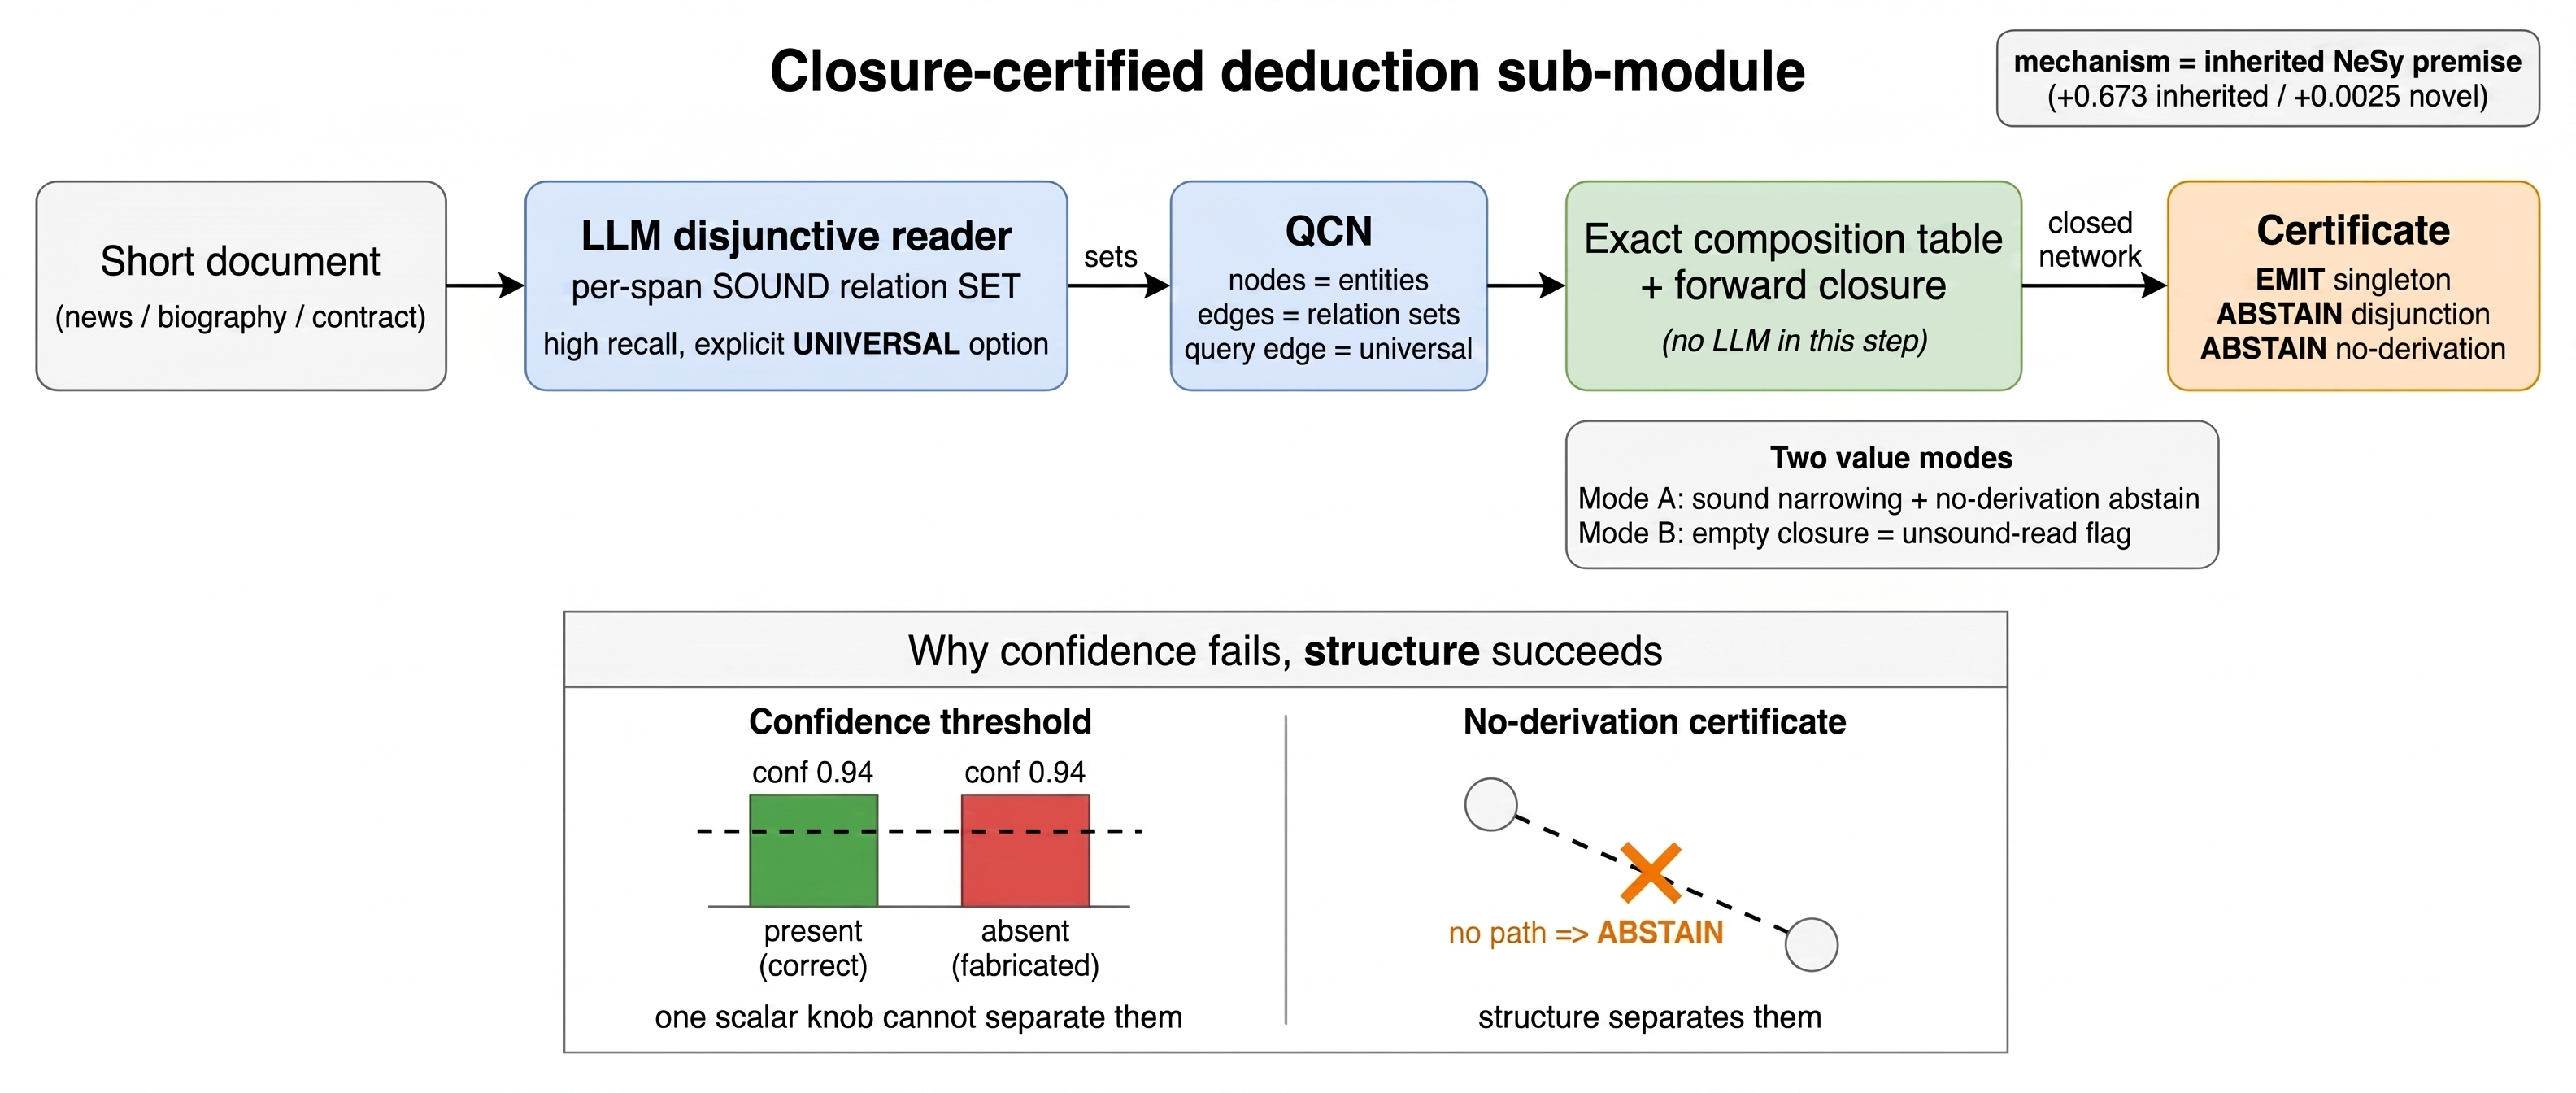
\includegraphics[width=\textwidth,height=0.45\textheight,keepaspectratio]{figures/fig1_v0.jpg}
  \caption{The closure-certified deduction sub-module of a text-to-logic pipeline. A high-recall disjunctive LLM reader emits a sound relation set per span; an exact composition table and forward closure narrow the held-out query edge; the system emits a singleton, abstains on a residual disjunction, or---the load-bearing case---abstains with `no relation' when no derivation path reaches the query. A confidence threshold cannot separate confident-present from confident-absent answers; the structural no-derivation certificate can.}
  \label{fig:fig1}
\end{figure*}

\subsection{Summary of Contributions}

\begin{itemize}
\item \textbf{A compositional false-premise diagnostic with a signal-agnostic capability gap} (Section~\ref{sec:diagnostic}). The raw LLM fabricates absent relations at high confidence in a $30$--$48\%$ band across CLUTRR and Re-DocRED, kinship and containment, and three readers, lifting the single-hop RE over-prediction of \citet{Yang2025DEPTH} to the compositional level. A $16$-cell per-signal $\times$ reader $\times$ corpus \emph{caught} table shows confidence-blindness is reader-dependent, not family-level; the reader-invariant spine is the mixed-pool capability gap, powered on CLUTRR (certificate selective accuracy $0.827$ vs.\ $0.37$--$0.44$; Holm-adjusted confident-wrong reductions $0.103$--$0.121$, all CIs exclude $0$) \footnote{Code: \url{https://github.com/AMGrobelnik/ai-invention-40a89b-no-derivation-no-relation-a-closure-cert/tree/main/round-8/evaluation-1}}.
\item \textbf{A no-derivation certificate that beats a query-side false-premise verifier---same-model and a stronger cross-family one} (Sections~\ref{sec:verifier}--\ref{sec:locatedin}). On a non-by-construction natural sibling-containment regime the certificate catches $0.785$ of high-confidence fabrications versus $0.274$ for the same-model verifier, $0.459$ for self-verify, and $\leq 0.40$ for every dispersion signal (all six certificate-minus-competitor caught-gaps exclude $0$) \footnote{Code: \url{https://github.com/AMGrobelnik/ai-invention-40a89b-no-derivation-no-relation-a-closure-cert/tree/main/round-9/evaluation-1}}. On its own $n{=}60$ subsample a stronger cross-family verifier (deepseek-v3.2, $k{=}5$) does \emph{worse} ($0.100$ vs.\ certificate $0.667$), because a better geographer over-infers co-regional containment \footnote{Code: \url{https://github.com/AMGrobelnik/ai-invention-40a89b-no-derivation-no-relation-a-closure-cert/tree/main/round-9/experiment-1}}. This is a targeting-quality win, paired throughout with the extraction-gated net-utility caveat.
\item \textbf{A structural net-utility boundary, established with a precision-preserving extractor} (Section~\ref{sec:boundary}). We build a trained, threshold-tunable extractor two ways (calibrated GBDT and fine-tuned DeBERTa-v3-small) \footnote{Code: \url{https://github.com/AMGrobelnik/ai-invention-40a89b-no-derivation-no-relation-a-closure-cert/tree/main/round-10/experiment-1}}. Both dominate the prompt-only frontier (the encoder reaches recall $0.65$ at precision $0.59$, strictly beyond the prompt-only ceiling of $0.23$), yet no operating point lifts the mixed-pool confident-wrong reduction above zero ($0$ sweet spots; best worst-case reduction $-0.001$). The certificate's own sibling confident-wrong rises in near-lockstep with present coverage and crosses above the fixed verifier baseline ($0.218$) at recall ${\approx}0.64$, because \textsf{located\_in} transitivity turns each recall-bought false edge into a spurious containment path. The gold-read ceiling stays $1.0/1.0/1.0$: the headroom exists but is not extractor-reachable.
\item \textbf{An end-to-end SWI-Prolog-executed CLUTRR pipeline} (Section~\ref{sec:clutrr}) delivering atomic P/R, multi-hop accuracy, runnable trace-graphs, and absent-relation safety, plus honest boundaries folded into a single feasibility appendix: cross-path coding is synthetic-only, natural temporal text is only weakly protective, and fuzzy unification / ${\sim}3000$-character operation are feasibility notes (Appendix~\ref{sec:feasibility}).
\end{itemize}

\begin{table}[t]
\centering
\small
\begin{tabular}{p{2.5cm}p{1.7cm}p{1.3cm}p{1.35cm}}
\hline
Claim & Evidence class & Where & Status \\
\hline
Compositional false-premise diagnostic + capability gap & real LLM read, 2 corpora / 2 domains / 3 readers & \S\ref{sec:diagnostic} & Robust; gap powered on clean graph \\
Certificate $>$ confidence battery \emph{and} query-side verifier (catching objective) & real LLM read & \S\ref{sec:verifier}, \S\ref{sec:locatedin} & Confirmed, incl.\ stronger cross-family \\
Net mixed-pool utility & real LLM read & \S\ref{sec:boundary} & Clean graph: yes; natural prose: extraction-gated \\
Net-utility boundary is structural (precision-preserving extractor) & supervised extractor + replay & \S\ref{sec:boundary} & \textbf{New: structural, deeper than prompt-only} \\
Closure/abstain mechanism is inherited & zero-spend decomposition & \S\ref{sec:diagnostic}, App.~\ref{sec:mechanism} & Conceded ($+0.673/{+}0.0025$) \\
Cross-path coding synthetic-only & gold-gate + synthetic & \S\ref{sec:boundaries} & Resolved negative \\
\hline
\end{tabular}
\caption{The paper's spine. Evidence-class tags live here, not inline in the prose.}
\label{tab:spine}
\end{table}

\section{Related Work}
\label{sec:related}

\textbf{Confident absent-relation fabrication in relation extraction.} Confident \emph{absent}-relation fabrication is a documented RE phenomenon: LLM extractors over-predict relations on entity pairs that bear none. \citet{Yang2025DEPTH} measure a $96.9\%$ relation rate on \textsc{no-relation} pairs in SciERC and counter it with dependency-aware simplification, hierarchical refinement, and an RLHF reward model; \citet{Li2024RelClassifier} pre-filter candidate pairs with a trained classifier on DocRED/Re-DocRED; \citet{Pi2025RelPrior} filter unrelated pairs with a binary relation prior. All three target a single-hop, schema-bound ``no label for this pair'' decision solved by better extraction, refinement, or filtering, not a verdict over \emph{composed} edges.

\textbf{Premise verification and structural correction against external structure.} The closest structural detectors verify premises against \emph{external} knowledge: \citet{Qin2026PremiseVerification} validate each premise of a logicalized query by retrieval-augmented generation over factual sources (training-free, logits-free, but KB-dependent), and \citet{Sansford2024GraphEval} check response triples against the provided context with a trained NLI model. A third, recent family corrects extraction structurally rather than by confidence: ontology-grounded post-extraction correction repairs or commits a labeling against an external ontology---\citet{Loconte2026PostExtractionCorrection} detect domain--range violations with ontology-derived symbolic rules and correct them via LLM calls (ontology-consistency up to $98.4\%$), and \citet{Chepurova2026Wikontic} and \citet{Feng2024OntologyGrounded} enforce Wikidata type and domain--range constraints over an extracted graph. The \emph{no-derivation certificate differs from all of these}: it is a per-query, gold-free, training-free abstention computed from deductive closure over the \emph{document-internal} relation graph, whereas premise verification and ontology-grounded correction repair or commit a labeling against \emph{external} structure (a KB, a context, or an ontology); we add no external knowledge and abstain rather than commit. The unanswerable / false-premise line \citep{Hu2023, Kirichenko2025, Wen2024, Kim2022, Yu2022} addresses sentence-level presuppositions with trained or prompt-based detectors. None of these targets a compositional, multi-hop, document-internal absent-relation premise detected gold-free, training-free, and without any external KB by deductive closure---the gap this paper fills \footnote{Code: \url{https://github.com/AMGrobelnik/ai-invention-40a89b-no-derivation-no-relation-a-closure-cert/tree/main/round-10/research-1}}. Our two-part delta is therefore a \emph{setting} (compositional, multi-hop, document-internal premise vs.\ single-hop schema-bound \textsc{no\_relation} and sentence-level false premises) and a \emph{method} (a gold-free, training-free, no-external-KB closure certificate vs.\ trained refiners, external-KB/RAG checks, NLI-vs-context, and ontology-grounded correction).

\textbf{Abstention by confidence vs.\ abstention by structure.} The selective-prediction family \citep{Geifman2017, Lin2022, Tian2023, Wang2022, Kadavath2022, Kuhn2023, Farquhar2024, Manakul2023} thresholds a dispersion or self-confidence scalar. We make the contrast empirical (Sections~\ref{sec:diagnostic}--\ref{sec:locatedin}) and keep scope honest: on ordinary single-path deduction, where dispersion is informative, the confidence baselines tie or beat the certificate. We instantiate the recognized query-side method---self-ask decomposition \citep{Press2022}, self-verification \citep{Weng2022}, P(True) self-evaluation \citep{Kadavath2022}---as an explicit baseline (Section~\ref{sec:verifier}) and show the certificate beats it.

\textbf{The consistency-enforcement neighborhood.} A zero-shot study reports that ILP consistency enforcement does not raise F1 \citep{Kougia2024}; the most recent global temporal-graph generator still ILP-commits to one label per pair \citep{Eirew2025}. Our neuro-symbolic neighbors all retain a commit objective: NeSTR repairs toward a single conclusion \citep{Liang2025}; TReMu commits code over dialogue memory \citep{Ge2025}; Fan and Strube commit one F1-maximizing Allen label \citep{Fan2025}; GDLLM classifies one relation per pair \citep{Zhao2025}. METRE trains a multi-label head \citep{Hu2024} but is F1-trained, carries no set through a composition table, and does not abstain. ``When Silence Is Golden'' \emph{trains} temporal abstention via chain-of-thought supervision \citep{Zhou2026}; ours is structural and training-free. BeDiscovER is a discourse evaluation suite \citep{Li2025}. None preserves a disjunction \emph{and} abstains on closure-collapse with a gold-free certificate.

\textbf{Closure over machine-extracted relations and qualitative reasoning.} SputLink computes temporal closure to densify TimeBank \citep{Verhagen2005}; CAEVO does global inference by cascaded sieves \citep{Chambers2014}; structured learning enforces transitivity \citep{Ning2017}. All commit to one consistent labeling and do not abstain. Allen's interval algebra \citep{Allen1983}, the convex point algebra \citep{Vilain1986}, RCC-8 \citep{Randell1992}, and the cardinal-direction calculus \citep{Frank1996, Ligozat1998} supply exact tables; Mackworth's path consistency \citep{Mackworth1977} iterates to a fixpoint and is complete for the convex point algebra and ORD-Horn \citep{Nebel1994} but only sound-but-incomplete for full Allen IA and RCC-8 \citep{Renz1999}. Chain-of-thought \citep{Wei2022} and self-consistency \citep{Wang2022} operate at the answer level; Logic-LM self-refines on solver crashes \citep{Pan2023} and LINC majority-votes formalizations \citep{Olausson2023}; Path-of-Thoughts \citep{Zhang2024} and backward chaining \citep{Kazemi2022} reason each path independently. Inducing composition rules to fit task accuracy \citep{Zhang2023, Zhu2023} optimizes data fit, not the algebraic laws needed for soundness. The discourse reading prompts of \citet{Wei2024} ground our span-local protocol; RuleTaker \citep{Clark2020} targets propositional entailment; Reiter's diagnosis \citep{Reiter1986} supplies the hitting-set machinery for the Mode-B repair we scope as future work; hallucination in generation is a broad concern \citep{Ji2022}. Our spatial venue uses SpaRTUN-style RCC-8 scenes \citep{Mirzaee2022}, with SpartQA \citep{Mirzaee2021} and StepGame \citep{Shi2022} as contrasts; the natural absent-relation corpora are built from Re-DocRED \citep{Tan2022}, the completeness-corrected re-annotation of DocRED \citep{Yao2019}. The supervised extractor we use to probe the net-utility boundary is standard, interchangeable structured-extraction plumbing---a calibrated gradient-boosted classifier \citep{Ke2017} and a fine-tuned encoder \citep{He2021}, the same role a constrained-decoding reader \citep{Geng2023} would play---and is not claimed as a contribution.

\section{Method}
\label{sec:method}

\subsection{The inverted output contract}

The deduction module sits downstream of atomic extraction: it receives, for each pair of mentions co-occurring in a span, the relation the text licenses, and must answer queries about pairs that do \emph{not} co-occur. We model the relations as a Qualitative Constraint Network (QCN): nodes are events/entities, each edge carries a \emph{set} of base relations from a finite composition system $\mathcal{A}$ (the disjunction the evidence does not exclude), and the held-out query edge starts at the universal set. Three commitments define the contract. First, the LLM is a disjunctive, high-recall reader: for each span it emits the maximal sound set the text does not exclude, with an explicit universal/underdetermined option, rather than committing to one relation. Second, composition and converse come from the exact published table of $\mathcal{A}$, never from the LLM. Third, the system narrows by closure and \emph{abstains} when the query edge remains a non-singleton, and \emph{flags an unsound read} when it collapses to the empty set. Table~\ref{tab:notation} fixes notation.

\begin{table}[t]
\centering
\small
\begin{tabular}{ll}
\hline
Symbol / term & Meaning \\
\hline
$\mathcal{A}$ & composition system (point:3; RCC-8:8; Allen:13; kinship/located-in: finite tables) \\
$r$ & per-edge recall, $P(\text{gold}\in\text{emitted set})$ \\
no-derivation & query unreachable by any composition path \\
FACT~A & raw-LLM confident absent-relation fabrication rate \\
caught & fraction of fabrications a method turns into abstention ($1-$survival) \\
capability gap & no scalar threshold both covers present and abstains on absent \\
sibling-absent & same component, share a parent, no valid derivation path \\
diffcomp-absent & different components (structural-by-construction absence) \\
confident-wrong (CW) & a committed (non-abstained) answer $\neq$ gold \\
matched cov. & every method scored at the same single-relation resolution rate \\
\hline
\end{tabular}
\caption{Notation and metrics used throughout.}
\label{tab:notation}
\end{table}

\subsection{Two value modes}

\textbf{Mode~A (sound narrowing and no-derivation abstention).} Composing the LLM's per-edge sets through the exact table and intersecting at the query pair, the system emits iff the result is a singleton, abstains iff a disjunction remains, and---the load-bearing case---abstains with ``no relation'' iff no composition path reaches the query. The intersection of sound sets is always sound, so under all-sound inputs Mode~A's output contains gold with probability exactly $1.0$; this survives path-consistency incompleteness. \textbf{Mode~B (detection).} An empty closure is a deductive certificate that some contributing read is unsound, with no gold labels. Both modes carry the silent-wrong-narrowing dual: if gold is omitted from a contributing set (recall failure), closure can narrow to a confident wrong singleton with no collapse---bounded per-edge by $(1-r)$.

\subsection{The definitional half and the empirical half}

A high-confidence, self-consistent fabrication survives any dispersion threshold by construction: if the model commits an absent relation with maximal confidence and zero answer-dispersion, no threshold tuned on that dispersion can single it out. This is definitional. The empirical, non-obvious questions---which we lead with---are how often the LLM emits absent-relation fabrications at high confidence, and how strongly that fraction varies by reader. The reader-invariant claim is geometric: a single scalar knob cannot separate confident-and-right (present) from confident-and-wrong (absent) when the LLM emits both at the same confidence, whereas a structural certificate separates them by whether a derivation path exists.

\subsection{Baselines: confidence battery and query-side false-premise verifiers}

Every certificate comparison includes two baseline families thresholded to the \emph{same} single-relation coverage object. (1) A confidence-thresholded raw-abstain battery: verbalized confidence; self-consistency vote-margin over $k{=}10$ samples; Kadavath's P(True); semantic-entropy negentropy over $k{=}10$ relation-clustered samples \footnote{Code: \url{https://github.com/AMGrobelnik/ai-invention-40a89b-no-derivation-no-relation-a-closure-cert/tree/main/round-6/experiment-1}}. (2) The recognized method for this failure mode, a query-side false-premise verifier. We run two prompt-based, zero-training variants on the \emph{same} reader---a \textsc{relatedness} verifier (``are $X$ and $Y$ related by $\langle$kinship$|$containment$\rangle$ at all?'' $\rightarrow$ abstain on \textsc{unrelated}) and a \textsc{self-verify} pass on the committed answer \footnote{Code: \url{https://github.com/AMGrobelnik/ai-invention-40a89b-no-derivation-no-relation-a-closure-cert/tree/main/round-8/research-1}}---and a stronger cross-family verifier (deepseek-v3.2 with $k{=}5$ self-consistency), reported on its own subsample. The certificate's claim is credible only if it matches or beats these verifiers at matched coverage.

\subsection{Two absent regimes (the decisive design choice)}

A natural absent-relation pair can be absent for two structurally different reasons. \emph{Different-component} absence: the two entities lie in disjoint connected components, so a sound closure derives the empty set almost by definition---abstention is structural-by-construction and carries no evidential weight. \emph{Same-component sibling} absence: the two entities lie in one connected component and share a containing parent, but no valid derivation path links them (two places in one region where neither contains the other, so the only relevant composition cell, $\textsf{located\_in}\circ\textsf{contains}$, is undefined). The certificate's abstention here is still a structural no-path determination but a non-trivial one: it requires the composition table, not mere disconnection. The sibling regime is decisive because the raw reader fabricates a containment on $30\%$ of sibling pairs versus only $6\%$ of different-component pairs, and a relatedness verifier is fooled by the shared parent \footnote{Code: \url{https://github.com/AMGrobelnik/ai-invention-40a89b-no-derivation-no-relation-a-closure-cert/tree/main/round-7/dataset-1}}.

\subsection{A precision-preserving extractor as an interchangeable component}

The atomic extractor is the binding lever on natural prose, and it is interchangeable. A gold-read ceiling (closure over gold atomic edges, queried edge ablated) reproduces $100\%$ of present golds and abstains on $100\%$ of absent pairs, so all net-utility headroom lives in extraction recall, not the certificate. To test whether a better extractor flips the boundary, we build a \emph{precision-preserving} extractor two independent ways and feed its edges into the frozen certificate engine. The task is binary $\textsf{located\_in}(i,j)$ over ordered gold-entity pairs co-occurring within a two-sentence window (no name-grounding step, isolating relation-extraction recall); a calibrated GBDT \citep{Ke2017} over ${\sim}30$ engineered per-pair features and a fine-tuned DeBERTa-v3-small encoder \citep{He2021} over marked windows both expose a precision-monotone threshold $\tau$ via isotonic calibration on a doc-disjoint fold. The extractor is not a contribution and not a trained \textsc{no\_relation} refiner in the sense of \citet{Yang2025DEPTH}; it is standard structured-extraction plumbing whose only role is to push extraction recall as far as supervised training allows and ask whether the certificate's net-utility win then transfers.

\subsection{Datasets and metrics}

\textbf{Templated end-to-end venue.} CLUTRR kinship \citep{Sinha2019}, standardized to gold graphs with typed atomic edges, held-out multi-hop queries (hops $2$--$10$), and within-document absent pairs; template-generated, short ($\leq 871$ chars). \textbf{Natural absent-relation corpora.} Re-DocRED \citep{Tan2022} kinship \footnote{Code: \url{https://github.com/AMGrobelnik/ai-invention-40a89b-no-derivation-no-relation-a-closure-cert/tree/main/round-6/dataset-1}} and geographic/administrative \emph{located-in} containment, the latter carrying the same-component-sibling regime. \textbf{Natural temporal corpora.} NarrativeTime \citep{Rogers2019, Cassidy2014}, TDDMan \citep{Naik2019}, MATRES \citep{Ning2018} \footnote{Code: \url{https://github.com/AMGrobelnik/ai-invention-40a89b-no-derivation-no-relation-a-closure-cert/tree/main/round-1/dataset-1}}. \textbf{Spatial venue.} SpaRP-PS1 RCC-8 scenes \citep{Mirzaee2022}. \textbf{Synthetic backbone.} Globally-consistent QCNs over point, Allen, RCC-8 \footnote{Code: \url{https://github.com/AMGrobelnik/ai-invention-40a89b-no-derivation-no-relation-a-closure-cert/tree/main/round-1/dataset-2}}. \textbf{Metrics}: FACT~A; per-signal $\times$ reader $\times$ corpus \emph{caught} fraction (matched-coverage-fair, same denominator); mixed-pool selective accuracy at matched coverage; confident-wrong rate always reported with coverage; atomic P/R (held-fixed control on the LLM-read arm, the binding lever for the supervised extractor); and, for fuzzy reads, expected calibration error (ECE).

\section{Experimental Setup}
\label{sec:setup}

Readers are \texttt{google/gemini-3.1-flash-lite} (primary, temperature $0$) and, for cross-family checks, \texttt{deepseek/deepseek-v3.2} and \texttt{mistralai/mistral-small-2603}; all LLM calls use a SHA-256 disk cache and a hard cost guard. The supervised extractor is trained doc-disjoint ($2{,}321$ training documents vs.\ $283$ evaluation documents; $72{,}906$ training pairs, $12{,}791$ positive; a leakage guard asserts disjointness) and adds no LLM spend---all six competitor predictions are replayed byte-identical from the merged cache ($18{,}722$ cache hits, $0$ calls; a snapshot assertion against the frozen iter-8 pool confirms $0$ mismatches over all $1{,}215$ records). Several zero-spend reproduction gates underpin the carried literals: an $80/80$-check re-analysis of the CLUTRR and natural-kinship batteries ($62$ genuinely recomputed), a $68/68$-check re-analysis recomputing every located-in / verifier literal from per-query rows, an $87/87$-check iter-10 re-analysis that builds the corrected tables and the stronger-verifier subsample \footnote{Code: \url{https://github.com/AMGrobelnik/ai-invention-40a89b-no-derivation-no-relation-a-closure-cert/tree/main/round-10/evaluation-1}}, and a $32/32$ gate confirming the rebuilt CLUTRR/Re-DocRED pools are byte-identical before any new spend \footnote{Code: \url{https://github.com/AMGrobelnik/ai-invention-40a89b-no-derivation-no-relation-a-closure-cert/tree/main/round-8/experiment-2}}. Document-clustered paired bootstraps use $B{=}10000$, Holm-adjusted. The QCN engine is unit-test gated: the Allen $169$-cell and RCC-8 $64$-cell tables match published cells with $0$ failures, convex-point completeness is confirmed against brute force, and an iteration-isolation test confirms \textsc{full}$=$\textsc{naive} at length $2$ and \textsc{full}$\neq$\textsc{naive} on $3$-hop chains. The located-in run reads $1{,}215$ queries over $283$ documents ($515$ present $=$ $400$ held-out $+$ $115$ never-annotated; $450$ sibling-absent; $250$ different-component-absent) at ${\sim}\$2.66$; the prompt-only extraction sweep and the stronger cross-family verifier added a one-time $\$1.21$; the kinship verifier run $\$0.14$; the CLUTRR battery $\$0.30$; the natural-kinship run ${\sim}\$1.5$; the supervised-extractor run $\$0$; cached re-runs $\$0$.

\section{Results}

\subsection{The compositional false-premise diagnostic}
\label{sec:diagnostic}

\textbf{FACT~A is robust across corpora, domains, and readers.} The raw LLM commits a confident absent-relation answer on a tight band of absent pairs: CLUTRR $47.2\%$ (gemini) / $48.3\%$ (deepseek); Re-DocRED kinship $32.6\%$ / $31.8\%$; Re-DocRED located-in sibling pairs $30.0\%$ (gemini, mean confidence $0.94$, $94.8\%$ at confidence $\geq 0.9$) / $43.8\%$ (mistral) \footnote{Code: \url{https://github.com/AMGrobelnik/ai-invention-40a89b-no-derivation-no-relation-a-closure-cert/tree/main/round-8/experiment-1}}. This is the over-prediction \citet{Yang2025DEPTH} document single-hop ($96.9\%$ on SciERC \textsc{no-relation} pairs), measured here at the compositional, document-internal level and shown to transfer; the contribution is the reframing and its transfer, not the existence of the rate (Figure~\ref{fig:fig2}).

\begin{figure*}[!t]
  \centering
  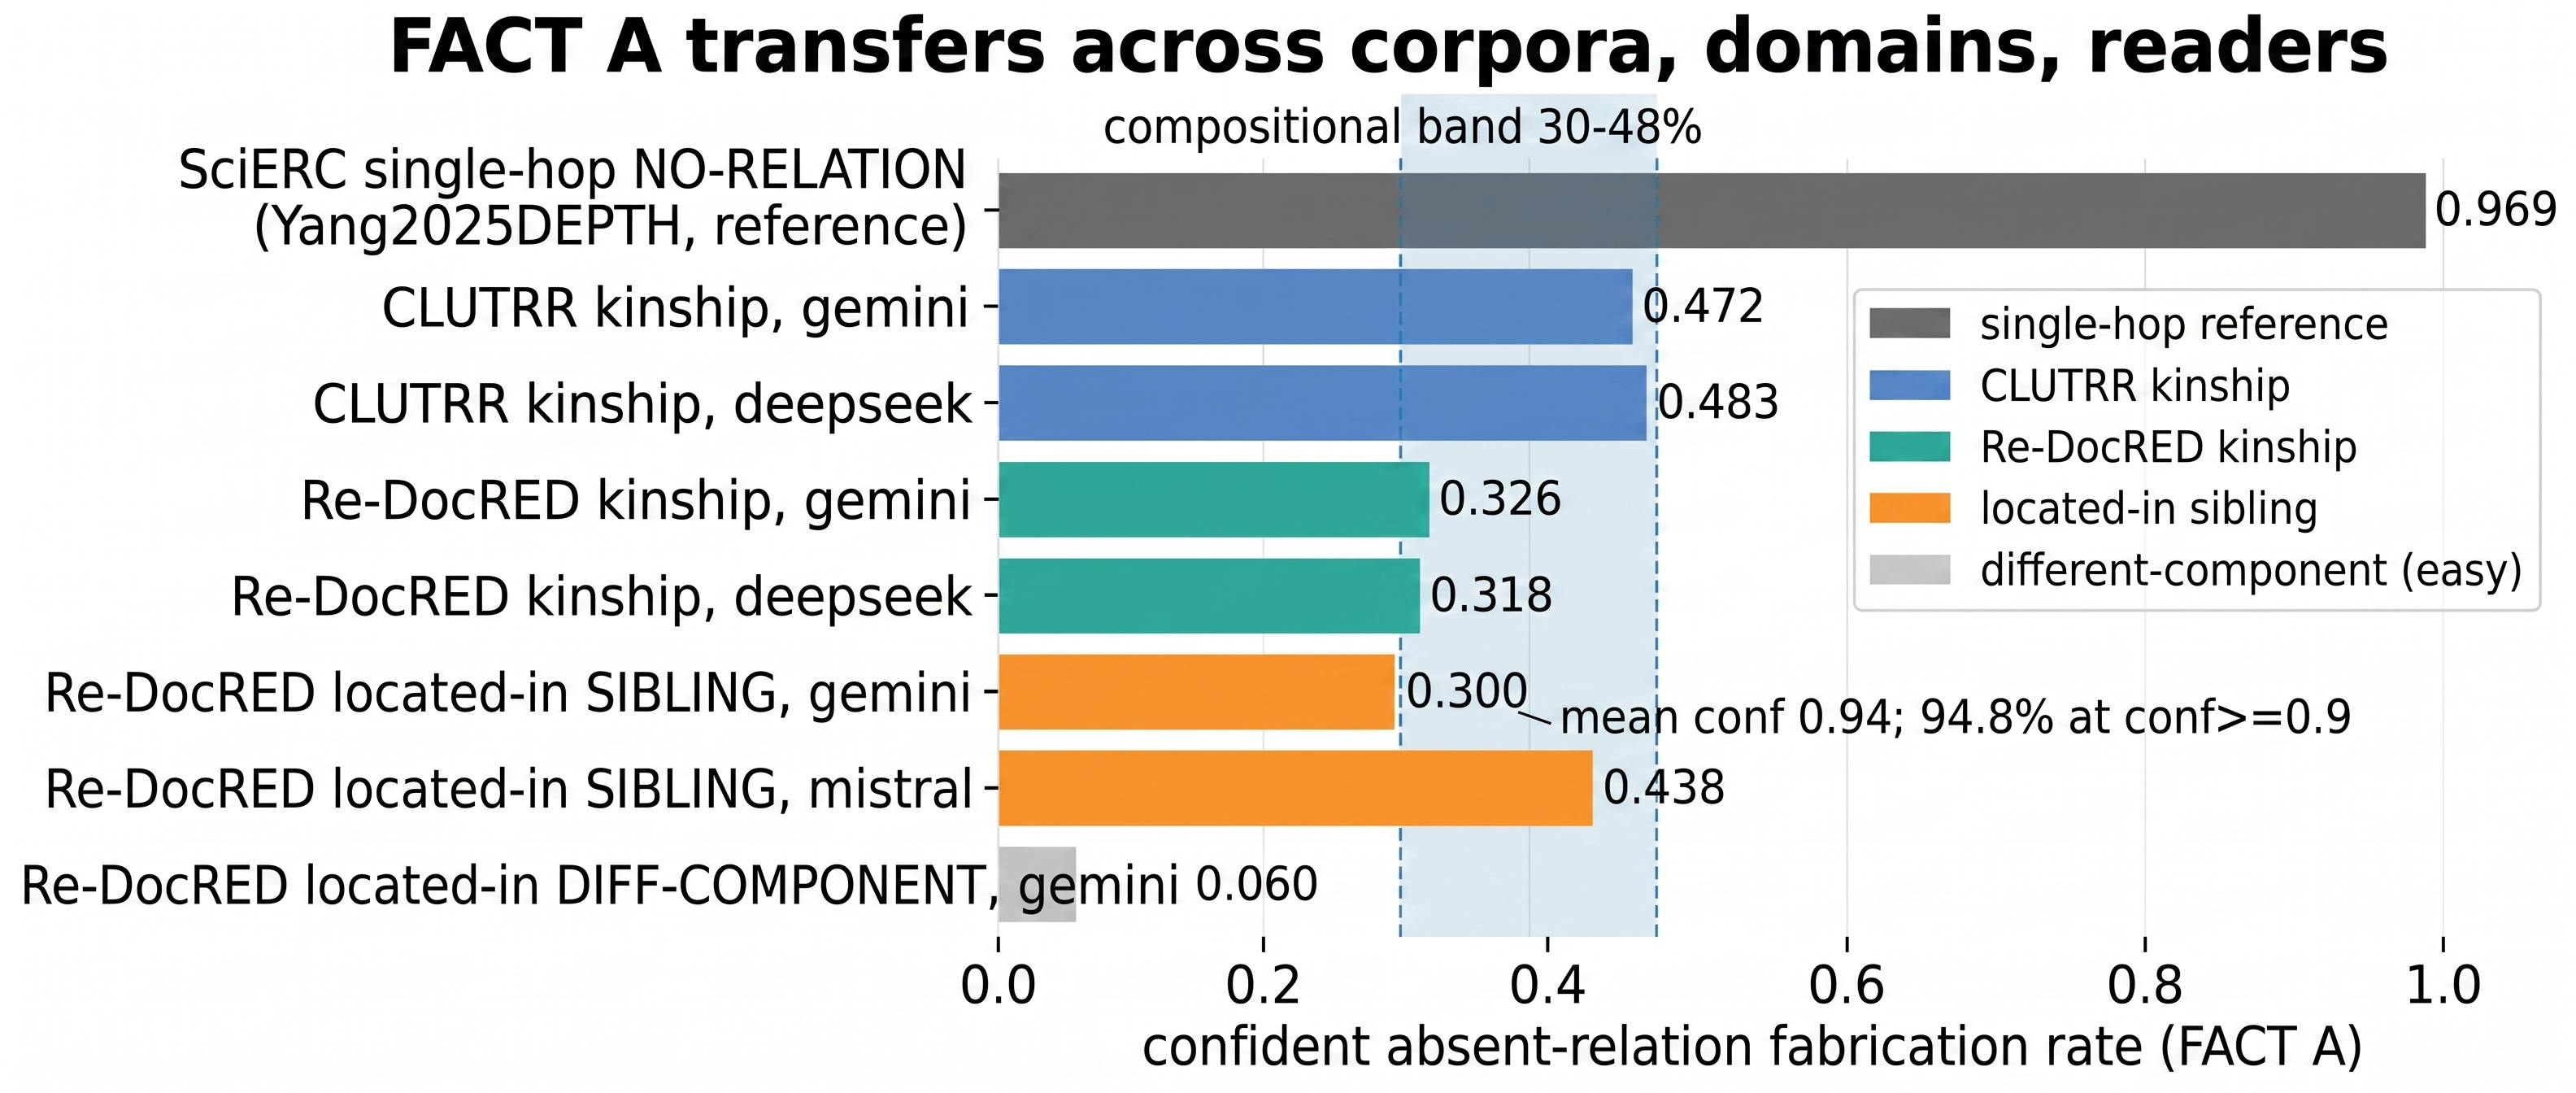
\includegraphics[width=\textwidth,height=0.45\textheight,keepaspectratio]{figures/fig2_v0.jpg}
  \caption{The raw LLM fabricates absent relations at high confidence in a tight 30--48\% band across CLUTRR and Re-DocRED, kinship and geographic containment, and three reader families, lifting the single-hop SciERC over-prediction (96.9\%) of Yang et al. to the compositional, document-internal level. Different-component absence (6\%) is the easy, structural-by-construction regime; the same-component sibling regime (30\%) is the hard one.}
  \label{fig:fig2}
\end{figure*}

\textbf{Whether a confidence signal can filter them is reader- and signal-dependent.} Table~\ref{tab:caught} reports, for four signals $\times$ two readers $\times$ two corpora, the fraction of fabrications a certificate-matched rule catches. The fraction swings from ${\sim}15\%$ (Re-DocRED/gemini, sc\_margin and negentropy) to ${\sim}90\%$ (CLUTRR/deepseek, P(True)): a practitioner using deepseek with self-consistency vote-margin already filters ${\sim}78\%$. We therefore do not claim family-level, reader-invariant blindness. The ``no signal removes a single fabrication'' statement holds only at the LLM's natural (no-abstention) coverage; at the certificate's coverage P(True) already catches $75.3\%$ on CLUTRR and $51.7\%$ on natural Re-DocRED (gemini). Verbalized confidence is the most robustly blind.

\begin{table}[t]
\centering
\small
\begin{tabular}{llccccc}
\hline
Corpus & Reader & FACT~A & verb. & sc\_marg. & P(True) & negent. \\
\hline
CLUTRR & gemini & 0.472 & 0.565 & 0.282 & \textbf{0.753} & 0.282 \\
CLUTRR & deepseek & 0.483 & 0.328 & 0.776 & \textbf{0.897} & 0.776 \\
Re-DocRED & gemini & 0.326 & 0.492 & 0.150 & 0.517 & 0.150 \\
Re-DocRED & deepseek & 0.318 & 0.588 & 0.706 & 0.676 & 0.706 \\
\hline
\end{tabular}
\caption{The $16$-cell per-signal $\times$ reader $\times$ corpus table of fraction \emph{caught} ($=1-$survival). FACT~A is reader-robust in a $0.32$--$0.48$ band; the caught fraction swings ${\sim}15\%$ to ${\sim}90\%$ by reader, so confidence-blindness is not family-level. The spine is the signal-agnostic capability gap, not per-signal blindness.}
\label{tab:caught}
\end{table}

\textbf{The signal-agnostic capability gap (the spine), powered on CLUTRR.} On a mixed present/absent pool ($n{=}282$, so abstaining-on-everything cannot win) at matched coverage $0.266$, the certificate's selective accuracy is $0.827$ versus verbalized $0.413$, sc\_margin $0.373$, P(True) $0.440$, negentropy $0.373$---roughly double every signal. Certificate-versus-signal confident-wrong reductions are $0.110$ (verbalized, Holm $p_{\text{adj}}{=}0.0004$), $0.121$ (sc\_margin, $0.0027$), $0.103$ (P(True), $0.0027$), $0.121$ (negentropy, $0.0027$), all CIs excluding $0$. A single neural threshold cannot simultaneously abstain on absent pairs and cover present ones; the certificate does both because its signal is structural. This capability gap is currently powered only on clean templated CLUTRR; Sections~\ref{sec:locatedin}--\ref{sec:boundary} test it on natural prose.

\subsection{A query-side false-premise verifier is not enough}
\label{sec:verifier}

The recognized method for false-premise abstention is a query-side verifier, not a dispersion threshold on a forced answer. On the absent-relation fabrication set (the pairs the raw LLM confidently committed), the fraction caught is, certificate vs.\ verifier vs.\ self-verify vs.\ best dispersion signal: CLUTRR $0.941$ / $0.588$ / $0.824$ / $0.753$; Re-DocRED $0.850$ / $0.100$ / $0.542$ / $0.517$. The certificate catches strictly more than the verifier on both venues (doc-clustered paired bootstrap $B{=}10000$; caught-gap $0.353$, CI $[0.187,0.510]$, and $0.750$, CI $[0.620,0.848]$, both excluding $0$, $p\leq 0.002$). The mechanism is the point: the verifier runs on the same LLM that hallucinated, so when the reader confidently invents ``$Y$ is $X$'s sister'' on an unrelated pair, asking ``are $X$ and $Y$ related?'' returns \textsc{related} at confidence $1.0$, inheriting the generation error, whereas the certificate's abstention is independent of the LLM's confidence.

\textbf{A stronger verifier does not close the gap.} We scope the necessity claim to a same-model prompt-based verifier and then test a stronger one. On a $250$-pair located-in sibling subsample carrying $60$ raw fabrications, a larger, different-family verifier (deepseek-v3.2 with $k{=}5$ self-consistency) catches only $0.100$ of the raw LLM's confident containment fabrications---worse than the same-model weak verifier ($0.200$ on this subsample) and far below the certificate ($0.667$)---because a better geographer over-infers containment between co-regional places (Table~\ref{tab:stronger}). This subsample carries a different denominator from the main pool of Section~\ref{sec:locatedin} and its numbers are not comparable to that pool's column; it is reported separately. Certificate-necessity is therefore not an artifact of a weak same-model verifier; the failure is intrinsic to running the premise check on a generative LLM.

\begin{table}[t]
\centering
\small
\begin{tabular}{lcc}
\hline
method (deepseek-v3.2, $k{=}5$; $n_{\text{sib}}{=}250$, $60$ fab.) & caught & nat.\ CW \\
\hline
\textbf{certificate (no-derivation)} & \textbf{0.667} & 0.096 \\
self-verification (strong) & 0.533 & 0.112 \\
query-side verifier (weak, same-model) & 0.200 & 0.192 \\
query-side verifier (strong, cross-family) & 0.100 & 0.216 \\
\hline
\end{tabular}
\caption{The stronger cross-family verifier on its \emph{own} $n{=}60$ subsample (separate denominator from Table~\ref{tab:locatedin}). A stronger, larger, different-family verifier is no better---in fact worse---and both verifiers sit far below the certificate. On this subsample the same-model verifier's value is $0.200$ (restricted to $n{=}60$), not the $0.274$ of the full pool; the two are kept in separate tables.}
\label{tab:stronger}
\end{table}

\subsection{The decisive non-by-construction catching test: located-in siblings}
\label{sec:locatedin}

We run the four-signal battery, the query-side verifiers, and the certificate on a second natural domain---Re-DocRED geographic containment---and, decisively, on the same-component sibling regime. A worked example: a Re-DocRED biography states that the A~Sau Valley is located in Thua~Thien-Hue Province (located in Vietnam) and is bisected by Route~548; asked ``what is the geographic relationship of the valley to Route~548?'', the gold is \textsf{no-relation} ($\textsf{located\_in}\circ\textsf{bisected-by}$ is undefined). The raw reader names a containment at high confidence; the certificate composes the extracted edges, finds no derivation reaching the pair, and abstains.

On the $450$ sibling-absent pairs, FACT~A is $30\%$, so $135$ pairs carry a high-confidence fabrication. Of those, the fraction each method turns into an abstention---computed on the same denominator---is: certificate $\mathbf{0.785}$, self-verification $0.459$, verbalized $0.400$, P(True) $0.304$, query-side verifier $0.274$, sc\_margin $0.067$, semantic-entropy $0.067$ (Table~\ref{tab:locatedin}). All six certificate-minus-competitor caught-gaps exclude $0$ (doc-clustered paired bootstrap $B{=}10000$). Under \texttt{mistral} the result is reader-general: FACT~A on siblings is $0.438$ and the certificate still catches ${\sim}78\%$ (Figure~\ref{fig:fig3}).

\begin{figure*}[!t]
  \centering
  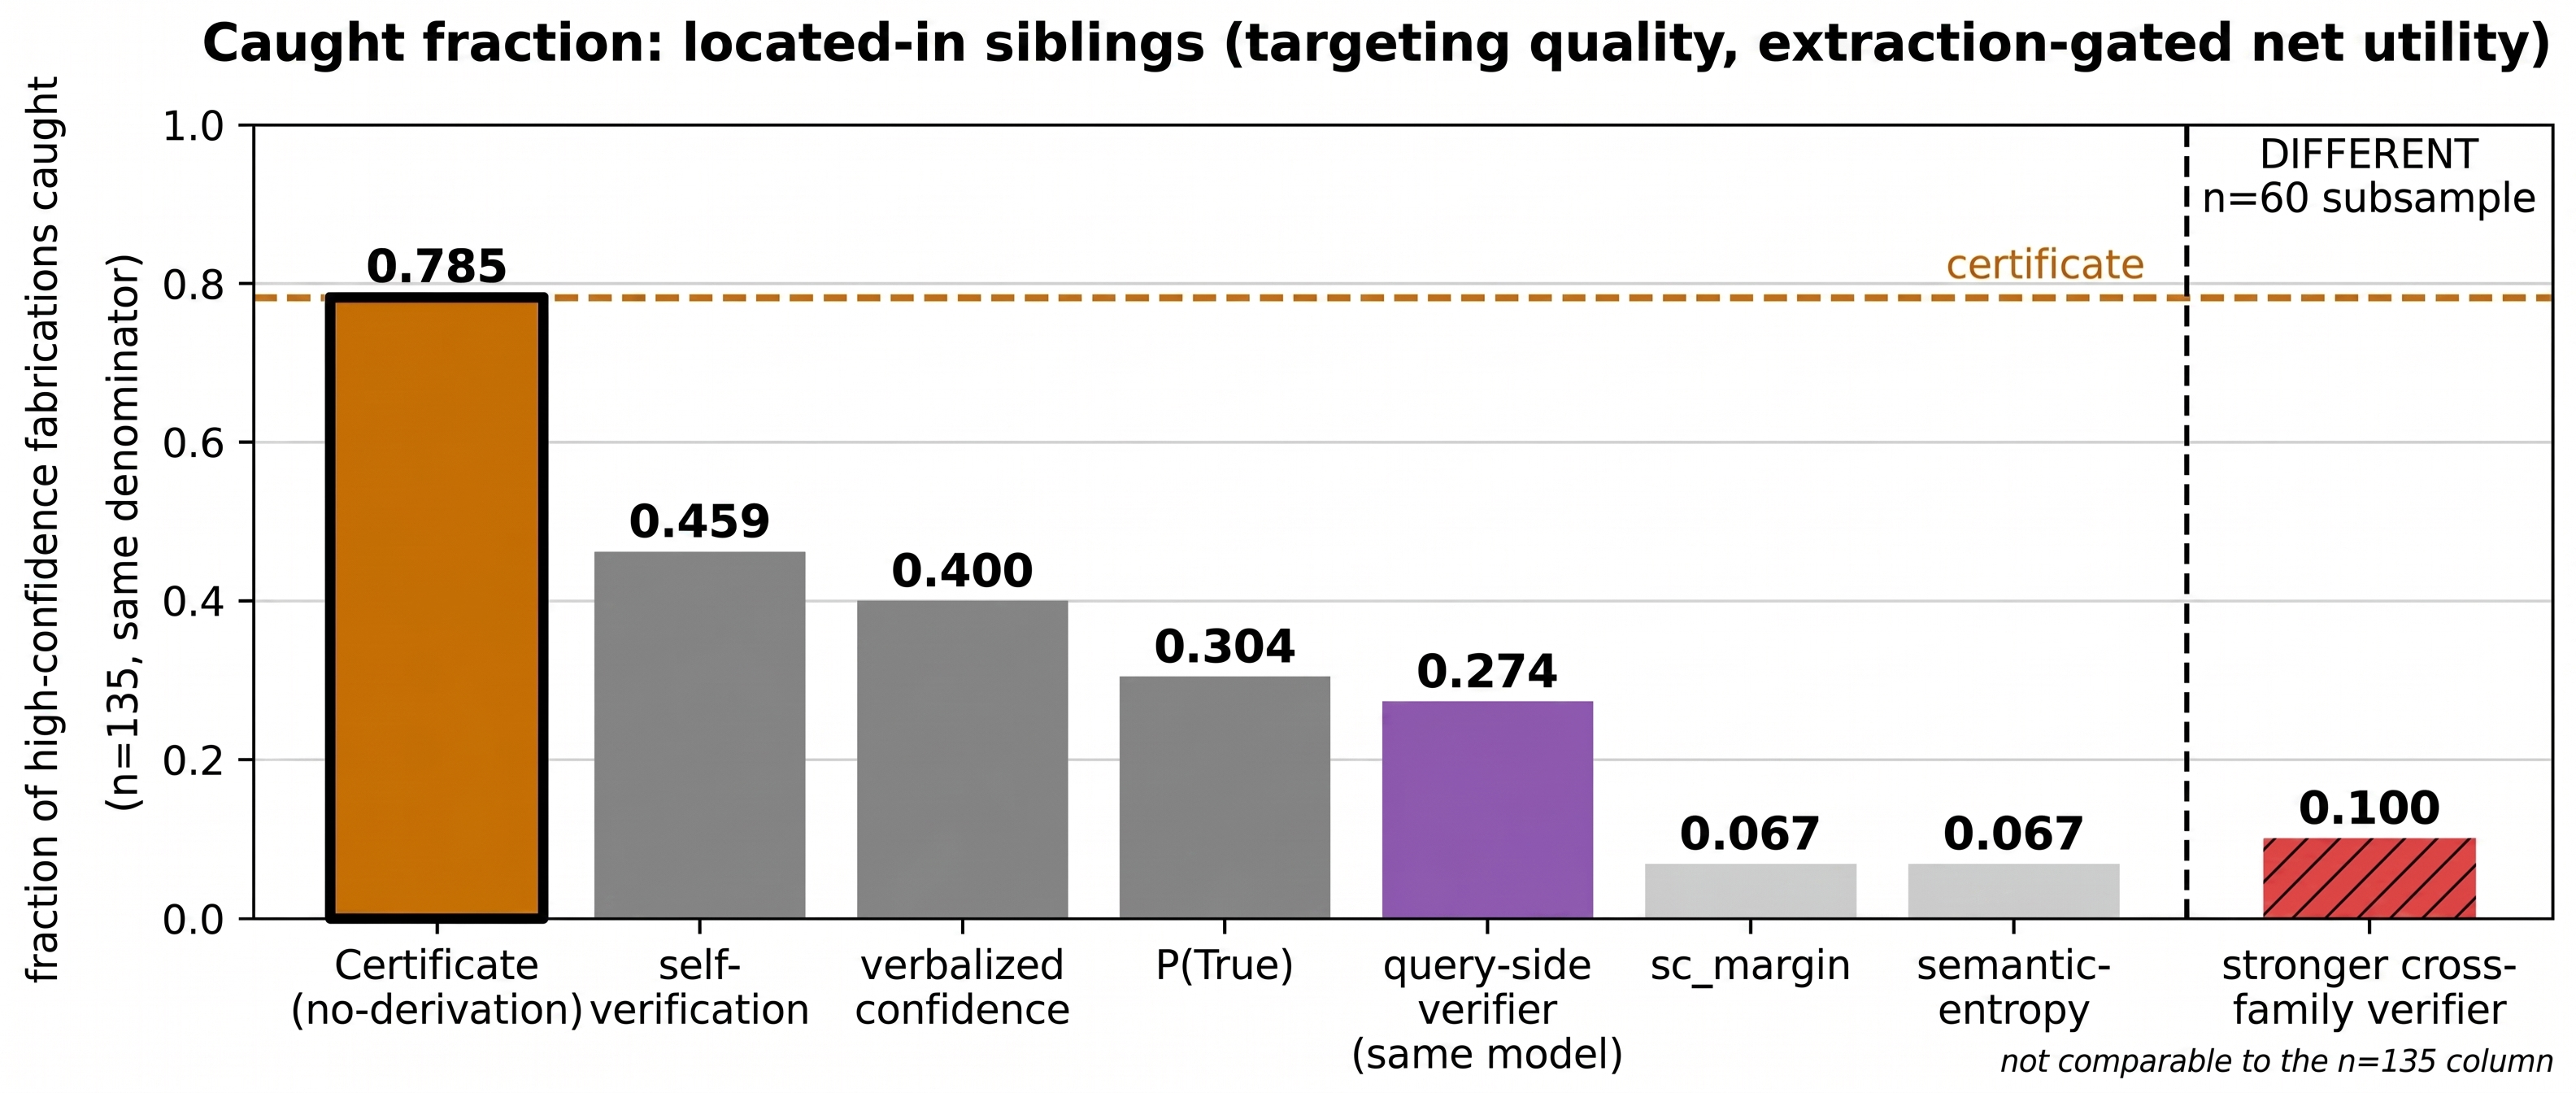
\includegraphics[width=\textwidth,height=0.45\textheight,keepaspectratio]{figures/fig3_v0.jpg}
  \caption{On Re-DocRED located-in same-component sibling pairs (n=450, FACT A 0.30, 135 fabrications), the no-derivation certificate turns 0.785 of the raw reader's high-confidence fabrications into abstentions versus 0.274 for the same-model query-side verifier and at most 0.40 for any dispersion signal, on the same denominator; all six certificate-minus-competitor gaps exclude 0. This is targeting quality, not a deployment win.}
  \label{fig:fig3}
\end{figure*}

\textbf{This is targeting quality, not a deployment win.} On a pure-absent pool every committed answer is wrong, so each method's natural confident-wrong rate equals its coverage: the certificate's is $0.073$ (it abstains on $92.7\%$) versus $0.30$ for the raw reader and every dispersion signal at its natural operating point, $0.218$ for the verifier, and $0.162$ for self-verify. The caught objective measures only how well a method's abstentions \emph{target} the fabrications, so it structurally rewards methods that abstain more on absent pairs; the deployment-relevant dual---net utility on a mixed present/absent pool---is exactly where the same structural abstention over-abstains on present pairs (Section~\ref{sec:boundary}). We therefore pair the $0.785$ result with the net-utility caveat wherever it appears: it establishes targeting quality, and the certificate's net utility on natural prose remains extraction-gated.

\begin{table}[t]
\centering
\small
\begin{tabular}{lccc}
\hline
Method & caught & cert$-$method gap & 95\% CI \\
\hline
\textbf{Certificate (no-derivation)} & \textbf{0.785} & -- & -- \\
self-verification & 0.459 & 0.326 & [0.207, 0.442] \\
verbalized confidence & 0.400 & 0.385 & [0.244, 0.520] \\
P(True) & 0.304 & 0.481 & [0.365, 0.596] \\
query-side verifier (same model) & 0.274 & 0.511 & [0.399, 0.620] \\
sc\_margin & 0.067 & 0.719 & [0.632, 0.800] \\
semantic-entropy & 0.067 & 0.719 & [0.632, 0.800] \\
\hline
\end{tabular}
\caption{The decisive non-by-construction test: Re-DocRED located-in same-component sibling pairs ($n{=}450$, FACT~A $0.30$, $135$ fabrications). Caught $=$ fraction of the raw LLM's high-confidence fabrications turned into an abstention, on the same denominator for every method; all six certificate-minus-competitor gaps exclude $0$. The stronger cross-family verifier ($0.100$) is on a different $n{=}60$ subsample (Table~\ref{tab:stronger}) and is deliberately absent here.}
\label{tab:locatedin}
\end{table}

\subsection{A precision-preserving extractor does not lift net utility: a structural boundary}
\label{sec:boundary}

The catching objective asks: among queries the raw LLM would answer with a fabrication, what fraction does the method abstain on? A stricter objective is \emph{net utility}: on a mixed pool of present and absent queries, improve selective accuracy at matched coverage---abstain on absent without over-abstaining on present. Net utility additionally requires high present coverage, which depends on extraction recall, and there the certificate is gated. On Re-DocRED kinship the certificate-versus-signal mixed-pool confident-wrong reductions are $-0.055$, $-0.034$, $-0.047$, $-0.034$, all CIs including $0$; mixed selective accuracy is certificate $0.475$ vs.\ signals $0.60$--$0.675$ \footnote{Code: \url{https://github.com/AMGrobelnik/ai-invention-40a89b-no-derivation-no-relation-a-closure-cert/tree/main/round-7/experiment-1}}. On located-in, the LLM-read present coverage collapses to $0.05$ because containment extraction recall is only $0.148$, so the certificate over-abstains on $94.9\%$ of present pairs. A gold-read ceiling settles attribution: closure over gold atomic edges reproduces $100\%$ of present golds and abstains on $100\%$ of absent pairs (present selective accuracy $1.0$), so the gap to the LLM-read certificate is the extraction ceiling, not the closure logic.

\textbf{The reviewer's fix, executed: a precision-preserving extractor.} A natural and reviewer-requested question is whether a better extractor flips this boundary, since the gold-read ceiling places the entire headroom in extraction. We replace the prompt-only LLM extractor with a trained, threshold-tunable extractor, built two independent ways (calibrated GBDT and fine-tuned DeBERTa-v3-small), and feed its edges into the frozen certificate engine at ten precision-preserving operating points; only the extraction step changes, and all six competitors are replayed byte-identical at $\$0$. The supervised extractor decisively escapes the prompt-only precision tax. At its reference threshold the encoder reaches atomic P/R/F1 $=0.738/0.589/0.655$ (recall $0.861$ against the locally-justifiable, span-extractable gold), and it \emph{dominates} the entire iter-9 prompt-only frontier: at every matched recall it has higher precision \emph{and} a less-negative net-utility CI-lower, and the encoder's lowest operating recall ($0.281$ at precision $0.929$) already exceeds the prompt-only ceiling ($0.227$), reaching a maximum recall of $0.650$ at precision $0.586$---a recall regime prompt-only never attained (Figure~\ref{fig:fig5}).

\begin{figure*}[!t]
  \centering
  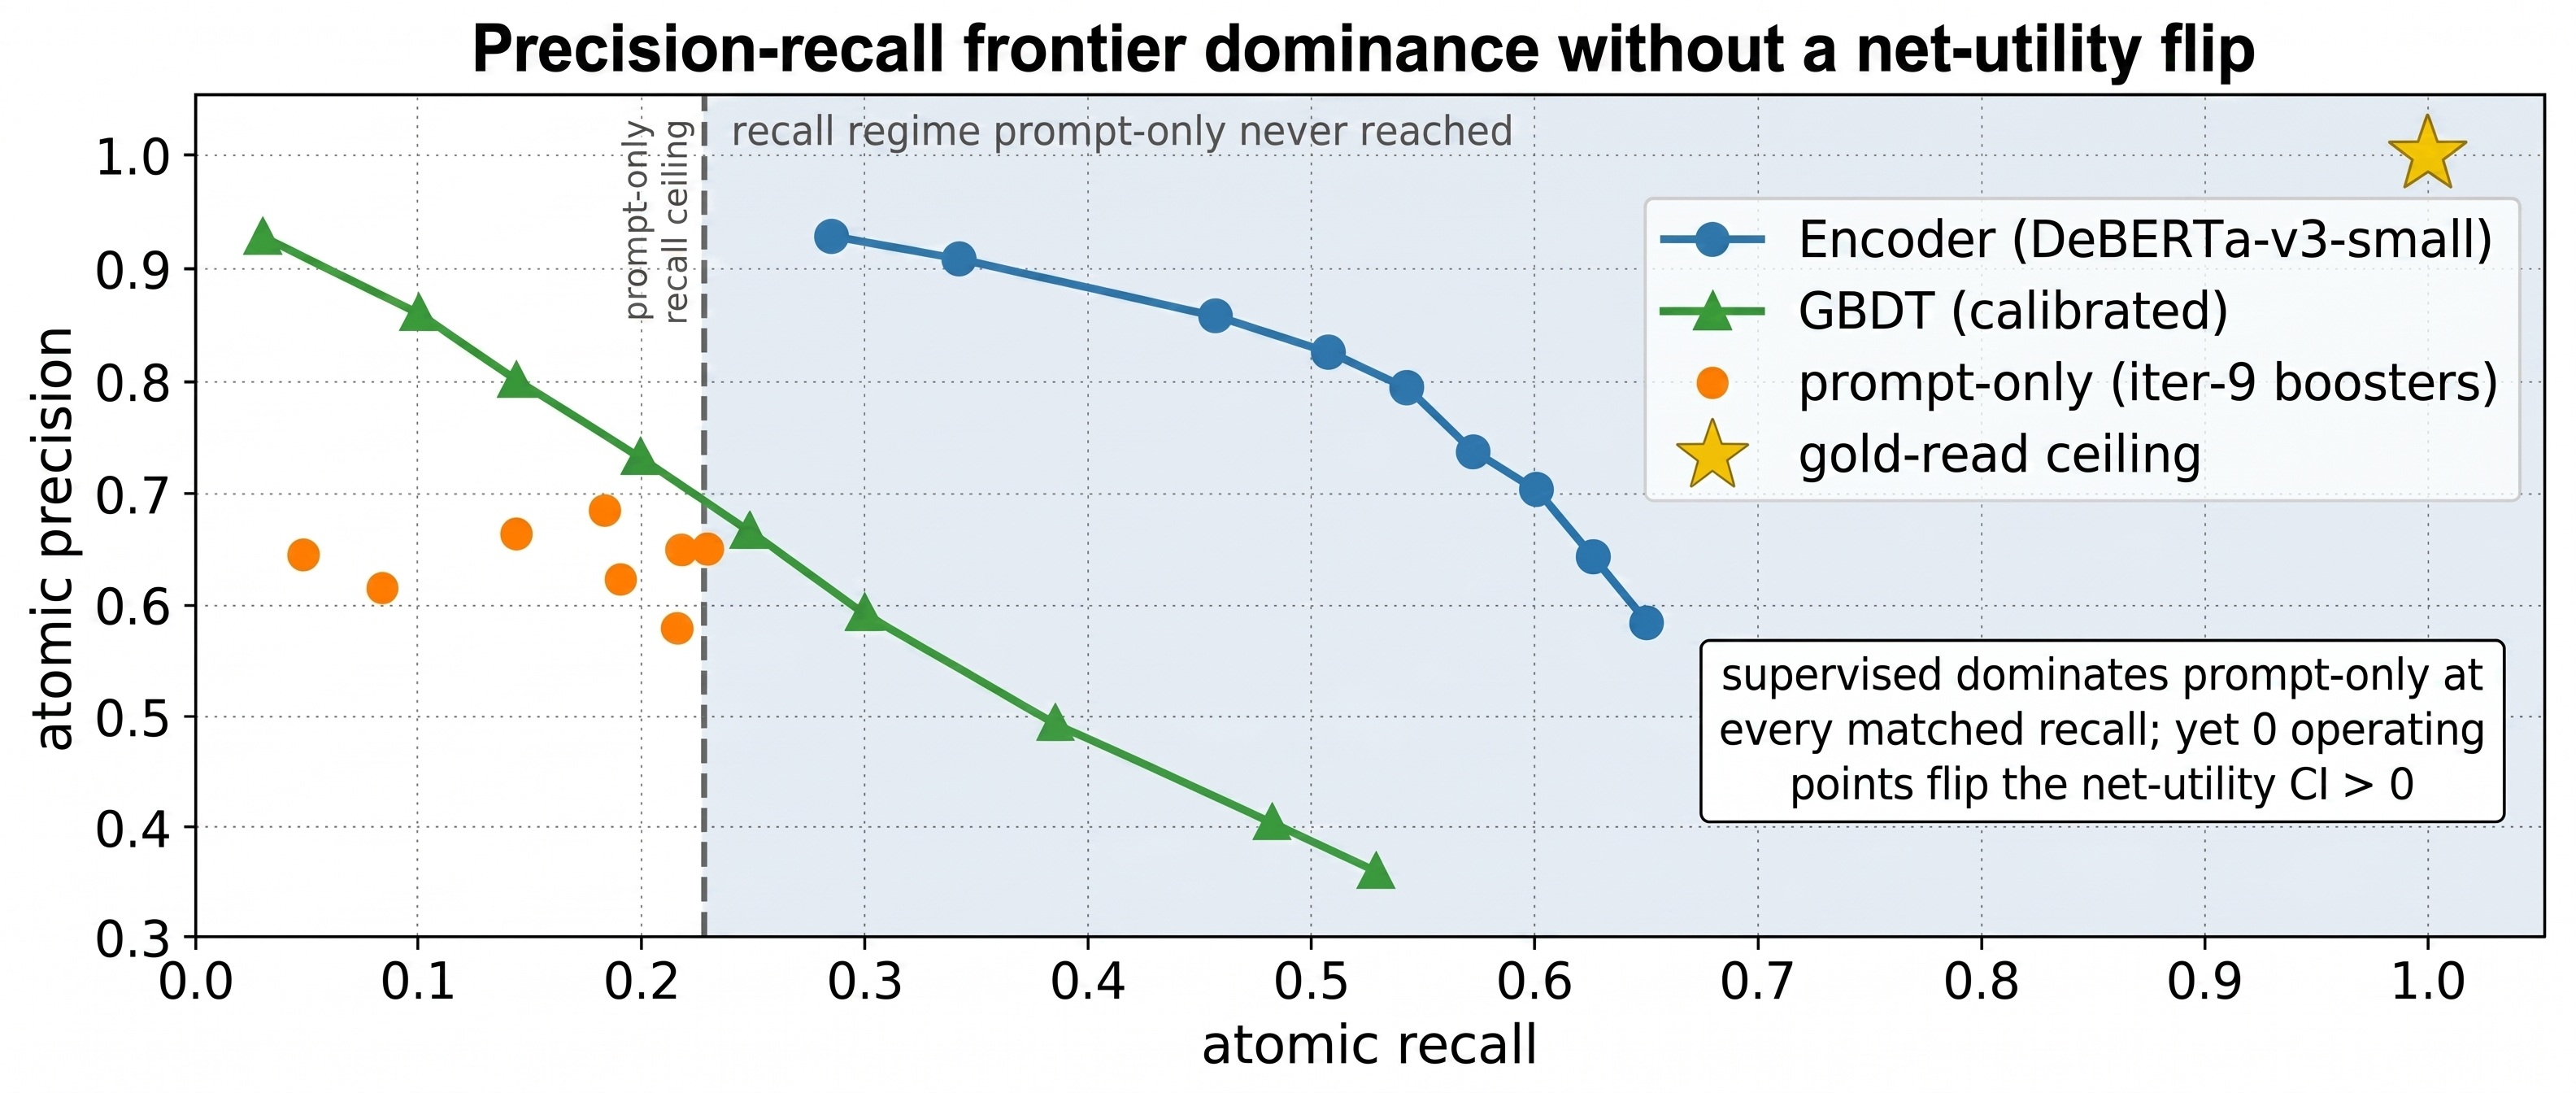
\includegraphics[width=\textwidth,height=0.45\textheight,keepaspectratio]{figures/fig5_v0.jpg}
  \caption{Atomic located\_in extraction precision vs.\ recall. Both supervised families (fine-tuned DeBERTa-v3-small encoder; calibrated GBDT) dominate the prompt-only frontier at every matched recall and operate strictly beyond its recall ceiling of 0.227, escaping the prompt-only precision tax. The gold-read point sits at (1.0, 1.0). Despite this dominance, no supervised operating point lifts the mixed-pool confident-wrong reduction above zero.}
  \label{fig:fig5}
\end{figure*}

\textbf{Yet no operating point flips the boundary, and the reason is structural.} Across both families and all ten thresholds, not one operating point lifts the worst-case (min-over-six-competitor) mixed-pool confident-wrong reduction above zero (best worst-case reduction $-0.001$, CI-lower $-0.0033$; $0$ sweet spots). The mechanism is read directly off the sweep (Table~\ref{tab:supervised} and the boundary figure, Figure~\ref{fig:fig4}). The query-side verifier's sibling confident-wrong is fixed at $0.218$ because it ignores the extracted graph. The certificate's sibling confident-wrong is far lower at high-precision points ($0.011$ at recall $0.281$) where it abstains structurally---but present coverage there is only $0.025$, so the throttled competitors commit almost nothing and there is nothing to beat. Raising recall to lift present coverage pushes the certificate's \emph{own} sibling confident-wrong up in near-lockstep---$0.327$ at recall $0.650$ (present coverage $0.565$), crossing above the verifier's fixed $0.218$ at recall ${\approx}0.636$---because $\textsf{located\_in}$ transitivity turns each injected sibling false-edge into a spurious containment path. The two requirements for a strict win, present coverage high enough to beat the throttled competitors \emph{and} sibling confident-wrong below the fixed verifier, are anti-correlated through extraction recall, so no operating point satisfies both. The gold-read ceiling stays $1.0/1.0/1.0$ throughout: the headroom is real but not extractor-reachable. The net-utility limit on this natural-prose regime is therefore structural---deeper than the refuted prompt-only boundary and not an extraction-quality artifact.

\begin{figure*}[!t]
  \centering
  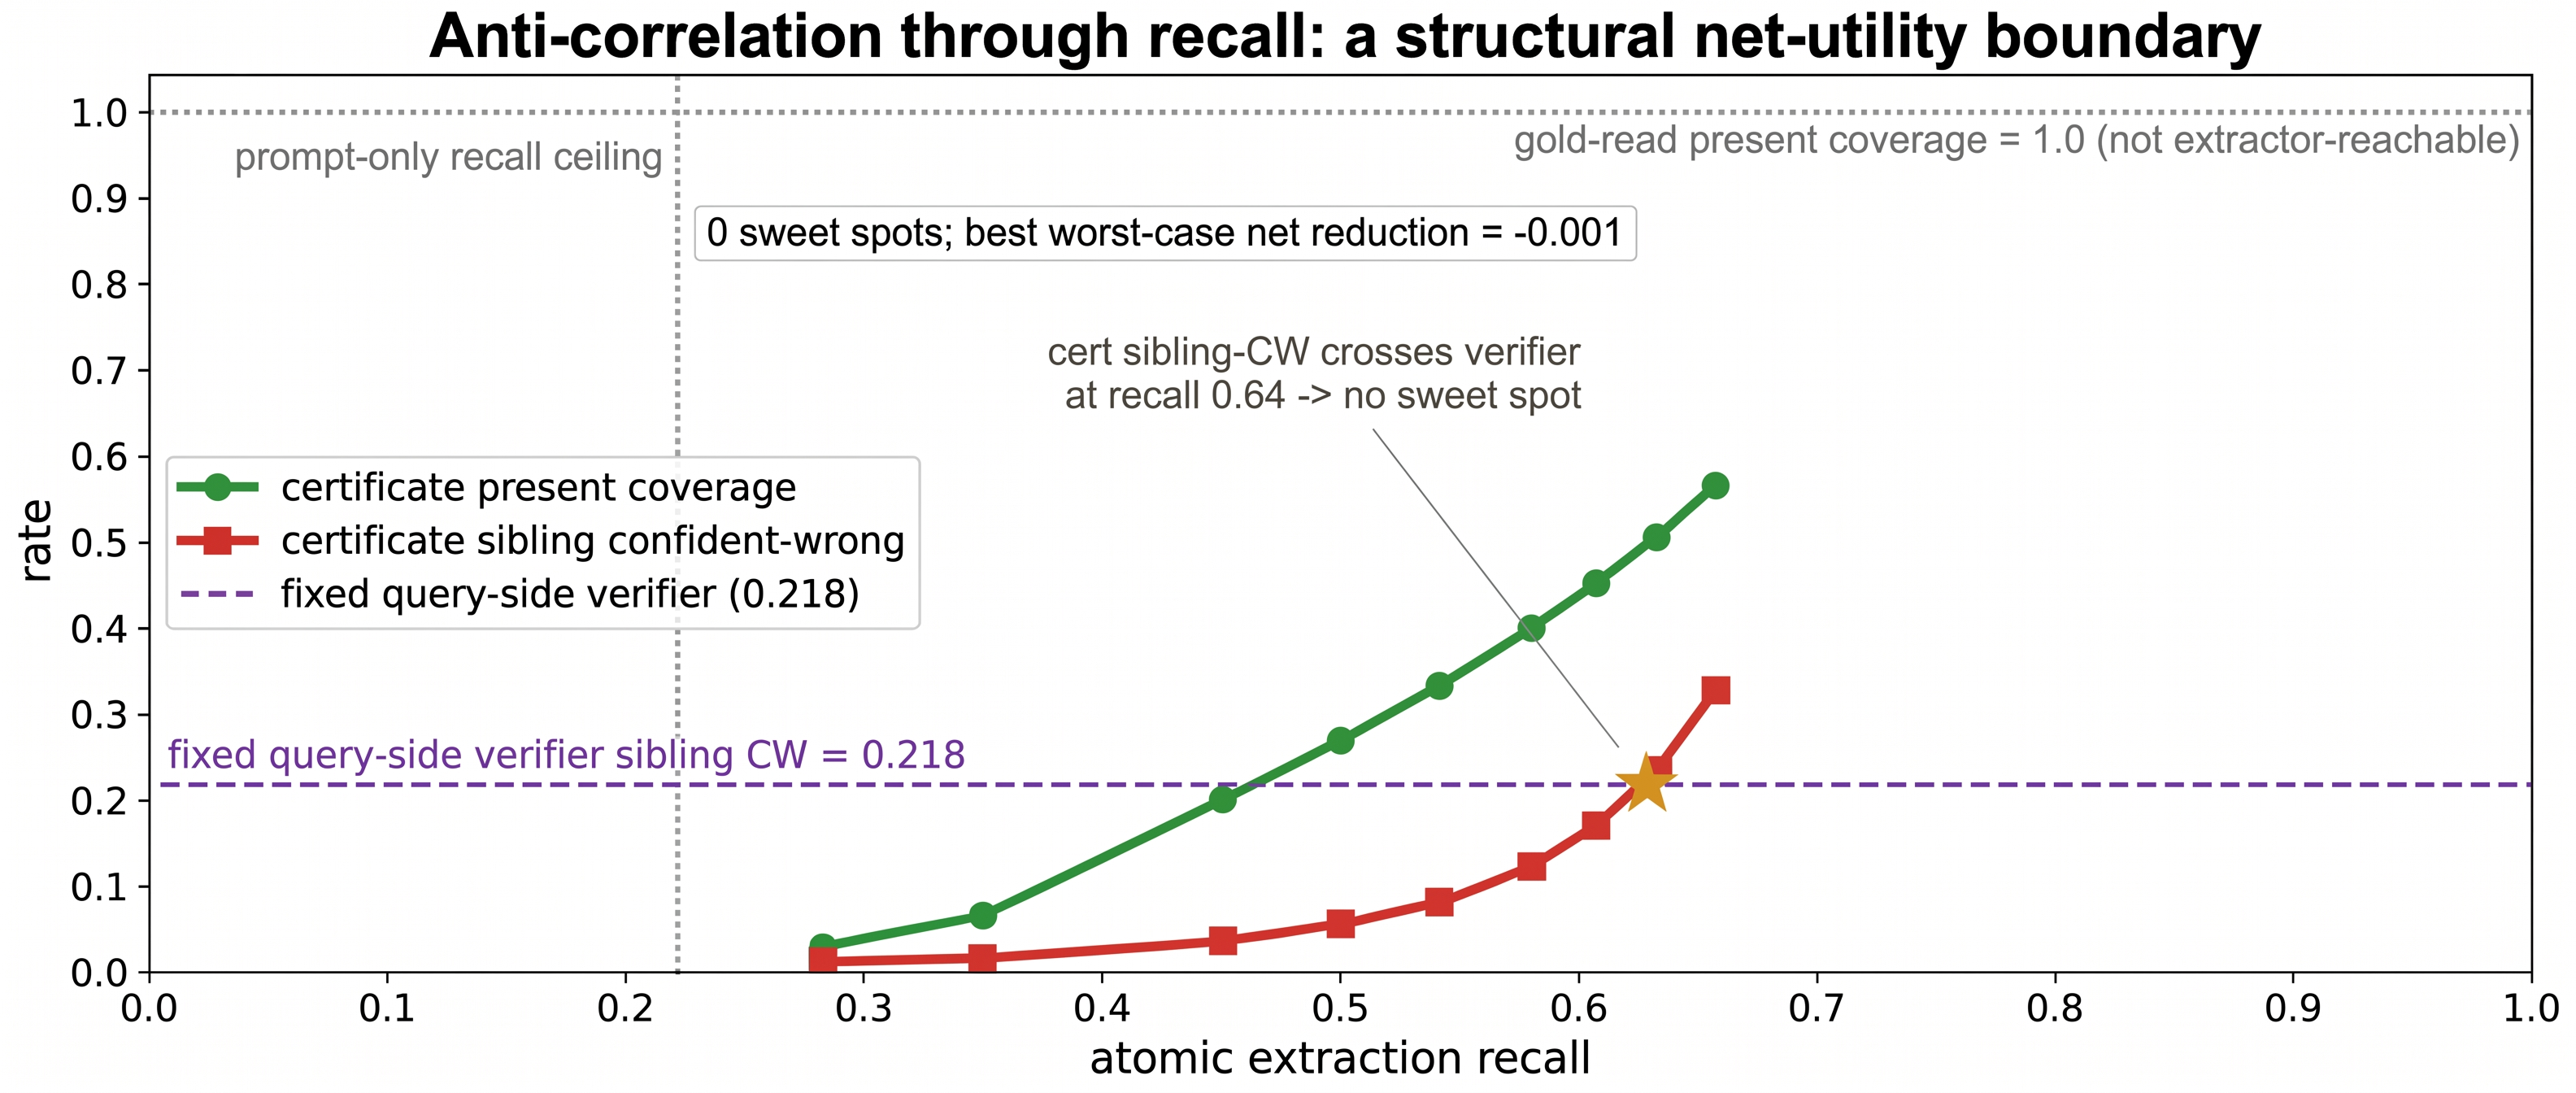
\includegraphics[width=\textwidth,height=0.45\textheight,keepaspectratio]{figures/fig4_v0.jpg}
  \caption{Sweeping the precision-preserving encoder extractor over thresholds. As atomic recall rises, the certificate's present coverage climbs (good), but its own sibling confident-wrong climbs in near-lockstep (bad), crossing above the fixed query-side verifier baseline (0.218) near recall 0.64, because located\_in transitivity turns each recall-bought false edge into a spurious containment path. The two win-requirements are anti-correlated through recall, so no operating point flips the mixed-pool reduction; the prompt-only ceiling (recall 0.227) and gold-read ceiling (1.0) bound the axis.}
  \label{fig:fig4}
\end{figure*}

\begin{table}[t]
\centering
\small
\begin{tabular}{lccccc}
\hline
Extractor / point & recall & prec. & pres.\ cov. & sib.\ CW & net redux (CI-lo) \\
\hline
gold-read ceiling & 1.000 & 1.000 & 1.000 & 0.000 & win (by constr.) \\
prompt-only default & 0.148 & 0.665 & 0.051 & 0.073 & $-0.034$ ($-0.050$) \\
encoder $\tau{=}0.95$ & 0.281 & 0.929 & 0.025 & 0.011 & $-0.005$ ($-0.014$) \\
encoder $\tau{=}0.8$ & 0.464 & 0.858 & 0.204 & 0.036 & $-0.017$ ($-0.028$) \\
encoder $\tau{=}0.4$ (best F1) & 0.589 & 0.738 & 0.400 & 0.122 & $-0.057$ ($-0.078$) \\
encoder $\tau{=}0.1$ & 0.650 & 0.586 & 0.565 & 0.327 & $-0.152$ ($-0.186$) \\
verifier (fixed) & -- & -- & -- & 0.218 & -- \\
\hline
\end{tabular}
\caption{The precision-preserving extractor sweep on the located-in mixed pool (encoder family; GBDT mirrors it). ``sib.\ CW'' is the certificate's confident-wrong on sibling-absent pairs; ``net redux'' is the worst-case (min-over-six) mixed-pool confident-wrong reduction with bootstrap CI-lower. The certificate's sibling CW rises in lockstep with present coverage and crosses the fixed verifier ($0.218$) near recall $0.64$; no operating point achieves a CI-lower above $0$.}
\label{tab:supervised}
\end{table}

\subsection{End-to-end on CLUTRR}
\label{sec:clutrr}

The certificate runs end-to-end on real (templated) CLUTRR text: a real LLM reads atomic kinship triples span-by-span, a forward-union least-fixpoint engine recovers the held-out query, and a certificate is emitted \footnote{Code: \url{https://github.com/AMGrobelnik/ai-invention-40a89b-no-derivation-no-relation-a-closure-cert/tree/main/round-3/experiment-1}}. As a zero-LLM go/no-go, the gold-atomic engine on all $16{,}131$ clean stories is $100\%$ accurate on every emitted answer at a $98.5\%$ singleton rate; the $1.5\%$ abstentions are genuine table ambiguities. Four deliverables follow: (i) the span-local reader extracts typed kinship triples at P/R/F1 $=0.536/0.532/0.534$; (ii) Mode~A's selective accuracy stays $0.75$--$1.00$ from hop-2 through hop-10 while the raw LLM collapses (hop-3 $0.444\rightarrow$ hop-10 $0.0$), and at matched coverage $0.686$ Mode~A reaches $0.886$ versus Path-of-Thoughts $0.457$ (gap $+0.429$, CI $[0.299,0.563]$, Holm $p_{\text{adj}}{=}0.0015$)---this present-pair win is the inherited premise; (iii) the closed network is discharged as runnable SWI-Prolog $9.0.4$ and executed: $40/40$ sampled programs run to exit $0$, $40/40$ match the Python engine, $39/40$ match gold; (iv) the absent-relation safety of Sections~\ref{sec:diagnostic}--\ref{sec:locatedin}, with a raw-vs-certificate confident-wrong reduction of $0.444$ (CI $[0.317,0.583]$) on absent pairs. A gold-read oracle ($1.00$ at coverage $0.951$) localizes the bottleneck to the neural read, not the closure. CLUTRR's $2.8\%$ confident-wrong on absent pairs is structural-by-construction (disconnected components) and never carries the contribution.

\subsection{Boundaries of the mechanism}
\label{sec:boundaries}

Two further results are honest negatives. \textbf{Cross-path coding is synthetic-only.} The most novel mechanism we explored---cross-path intersection of disjunctive reads as an error-correcting code over LLM extractions---does not transfer to real text, because each of its two preconditions was independently violated on the two venues we could gate before any LLM spend. Temporal Allen reads are near-universe (underdetermined rate $0.87$; the stronger deepseek is more conservative at $0.99$), so intersection, best-single, and naive all resolve $0/125$ \footnote{Code: \url{https://github.com/AMGrobelnik/ai-invention-40a89b-no-derivation-no-relation-a-closure-cert/tree/main/round-4/experiment-1}}; the spatial RCC-8 subgraph is a containment tree (all $228$ queries have one edge-disjoint path) \footnote{Code: \url{https://github.com/AMGrobelnik/ai-invention-40a89b-no-derivation-no-relation-a-closure-cert/tree/main/round-5/experiment-1}}. Synthetic controls satisfying both conditions confirm the mechanism is real (Allen intersection selective accuracy $0.976$ vs.\ best-single $0.717$, $+0.259$, CI $[0.177,0.349]$; RCC-8 $0.890$ vs.\ $0.797$). \textbf{Natural temporal text is only weakly protective.} Scaling to $600$ deduction-required queries in the PC-complete convex point algebra, the Mode-A advantage is marginal and not robustly significant (vs.\ Path-of-Thoughts $+0.027$, CI $[-0.088,0.140]$, $p{=}0.33$; vs.\ self-consistency $+0.035$, CI $[-0.061,0.135]$, $p{=}0.26$; neither clears Holm; the raw LLM is in fact more accurate than Mode~A at this coverage, $0.699$ vs.\ $0.575$); among the $18.8\%$ of queries Mode~A commits, $42.5\%$ are confident-wrong, all silent-wrong-narrowing \footnote{Code: \url{https://github.com/AMGrobelnik/ai-invention-40a89b-no-derivation-no-relation-a-closure-cert/tree/main/round-3/experiment-2}}\footnote{Code: \url{https://github.com/AMGrobelnik/ai-invention-40a89b-no-derivation-no-relation-a-closure-cert/tree/main/round-4/evaluation-1}}. A synthetic backstop closes the loop: when reads are sound (recall $0.96$), Mode~A beats raw by $+0.225$ at matched coverage \footnote{Code: \url{https://github.com/AMGrobelnik/ai-invention-40a89b-no-derivation-no-relation-a-closure-cert/tree/main/round-2/experiment-2}}, isolating read-soundness, not closure, as the gate.

\section{Discussion}
\label{sec:discussion}

\textbf{What the evidence supports.} The compositional false-premise diagnostic holds as a robust empirical fact: the raw LLM fabricates absent relations at high confidence in a $30$--$48\%$ band across two corpora, two relational domains, and three readers---the compositional, document-internal lift of a single-hop RE phenomenon \citep{Yang2025DEPTH}---and no single confidence threshold can both cover present pairs and abstain on absent ones. We do not claim family-level, reader-invariant per-signal blindness; the $16$-cell table shows the dispersion signals catch a majority of fabrications for the stronger reader. Onto this diagnostic the structural certificate converts the geometry into a measurable safety advantage: it beats the confidence battery, the same-model query-side verifier, and a stronger cross-family verifier, and catches $78.5\%$ of high-confidence fabrications on a non-structural-by-construction natural containment regime where every dispersion signal catches $\leq 40\%$ and the verifier $27\%$. This catching win is targeting quality: it establishes that the certificate's abstentions are aimed at the right pairs, not that the certificate is net-deployable on mixed natural prose.

\textbf{What it does not support, and why the boundary is now deeper.} The certificate's full mixed-pool net utility is bounded on natural prose: extraction recall is low, so the certificate over-abstains on present pairs and ties or loses the matched-coverage showdown there. The new and stronger result is that this boundary survives the obvious fix. A precision-preserving extractor, built two ways and dominating the prompt-only recall--precision frontier, still produces no net-utility flip, because $\textsf{located\_in}$ transitivity makes present coverage and the certificate's own sibling errors rise together: the very recall that recovers non-local present-path edges injects sibling false-edges that re-create spurious containment paths. The two win-requirements are anti-correlated through recall, and the gold-read ceiling ($1.0/1.0/1.0$) shows the headroom is real but not extractor-reachable on this regime. The limit is therefore structural to natural-prose located-in extraction, deeper than the prompt-only boundary, and we report it as the central caveat rather than a future-work hope. The certificate mechanism itself is the inherited neuro-symbolic premise ($+0.673$ inherited / $+0.0025$ novel), not our discovery; the cross-path coding mechanism is synthetic-only; and the natural-temporal advantage is marginal because recall-driven silent narrowing is undetectable.

\textbf{Where to deploy, and why.} Deploy the certificate wherever confident absent-relation queries carry real cost \emph{and} the relational graph either is clean (CLUTRR-like or semi-structured inputs) or composes without the transitive false-edge amplification that defeats located-in (a kinship-style table without a single dominant transitive relation is less exposed). There a confidence threshold and a query-side verifier both fail and the structural signal succeeds. Where extraction recall is low and the relation is strongly transitive, the diagnostic still tells operators that neither the confidence family nor a same-model (or stronger) verifier will catch confident absent-relation fabrications, and that the engineering lever is per-edge read-soundness in a non-amplifying relation, not more consistency post-processing or a better-calibrated threshold.

\textbf{Limitations.} (1) The certificate's mixed-pool net-utility win is powered only on templated CLUTRR; on natural Re-DocRED kinship and located-in it is extraction-limited, and a precision-preserving extractor does not lift it---on located-in the limit is structural (transitive false-edge amplification). (2) The cross-path coding mechanism is synthetic-only. (3) Path consistency is complete only for the convex point algebra; Allen and RCC-8 numbers are sound lower bounds. (4) No benchmark document reaches ${\sim}3000$ characters (natural prose averages ${\sim}1025$); the operational note's documents are bracket-selected (Appendix~\ref{sec:feasibility}). (5) Upper-ontology grounding, atomic re-extraction, and general open-vocabulary fuzzy unification are out of scope. (6) A third-party trained false-premise detector (FalseQA-style; a DEPTH-style RE refiner) is not run head-to-head and is future work; our verifier baselines are prompt-based (same-model and a stronger cross-family judge). (7) The structural boundary is established on located-in containment; whether a non-transitive natural relation admits a net-utility win is open.

\section{Conclusion}
\label{sec:conclusion}

We treated the deduction sub-module of a text-to-logic pipeline as a faithfulness problem and reframed its most damaging error---confident fabrication of a relation that does not exist---as a compositional false-premise failure, lifting a documented single-hop relation-extraction phenomenon to the compositional, document-internal level. The new knowledge is a diagnostic, a contrast, and a boundary. The raw LLM fabricates absent relations at high confidence robustly across corpora, domains, and readers; no single confidence threshold can both cover present and abstain on absent; and a gold-free, training-free, no-external-KB no-derivation certificate catches these fabrications where the confidence family and a query-side false-premise verifier (same-model and a stronger cross-family judge) do not, catching $0.785$ versus $0.274$ and $\leq 0.40$ on a non-by-construction natural containment regime---a targeting-quality result, not a deployment win, because the pure-absent catching objective favors high-abstention methods. We concede the certificate's machinery as the inherited neuro-symbolic premise, and we sharpen the boundary rather than soften it: a precision-preserving extractor, built two ways and dominating the prompt-only recall--precision frontier, still yields no net-utility flip on natural located-in prose, because the relation's transitivity converts every recall-bought false edge into a fabricated containment path, while a gold-read ceiling of $1.0/1.0/1.0$ shows the headroom exists but is not extractor-reachable. Three next steps follow: (1) test the certificate's mixed-pool advantage on natural \emph{non-transitive} relations, where the structural false-edge amplification we identify should not arise; (2) evaluate against a third-party trained false-premise / RE-NA detector head-to-head; and (3) integrate the validated certificate into a full pipeline with upper-ontology grounding.

\appendix

\section{Feasibility on commodity hardware}
\label{sec:feasibility}

Both notes below are feasibility demonstrations on commodity hardware, not substantive contributions; the substantive contributions are the diagnostic, the targeting-quality catching win, and the structural net-utility boundary.

\textbf{A.1 Operational ${\sim}3000$-character case study.} The full pipeline runs end-to-end on $5$ bracket-selected NarrativeTime articles (mean $3050$ chars), discharging and executing $95$ Prolog programs ($60$ temporal $+$ $35$ kinship) in SWI-Prolog $9.0.4$, with hallucination reduction $0.27$--$0.60$ (mean $0.45$) at Mode-A coverage $0$--$0.33$ and atomic recall ${\sim}0.49$ the binding ceiling \footnote{Code: \url{https://github.com/AMGrobelnik/ai-invention-40a89b-no-derivation-no-relation-a-closure-cert/tree/main/round-5/experiment-3}}. We cut the concatenated-kinship arm because its $56/56$ cross-story abstentions are trivial by construction. The documents are bracket-selected; the note establishes that the pipeline \emph{runs} at length, not that it is \emph{useful} at length.

\textbf{A.2 Genuine fuzzy unification.} In two labeled settings (vague spatial RCC-8; ambiguous kinship) a real LLM emits a calibrated disjunction over a known base vocabulary (fraction at confidence $1.0$ is $0.00$ in both, versus $1.00$ for the memorized-table recall a prior version mislabeled fuzzy unification; per-candidate ECE $0.142$ spatial / $0.111$ kinship), and the abstain-on-collapse certificate runs unchanged: all $5$ sound-violating spatial reads were caught (e.g.\ \textsf{around}$\rightarrow\{\textsf{NTPPi},\textsf{TPPi}\}$ drops gold \textsf{EC}, so closure collapses and the certificate abstains), with $0$ silent-wrong missed; the kinship arm had $0$ unsound reads, so its catch is untested. A supporting query-level comparison gives certificate confident-wrong $0.000$ vs.\ commit-argmax $0.364/0.216$ (CIs exclude $0$), with a query-vs-edge unit-of-analysis caveat. The note establishes feasibility, not upper-ontology grounding or open-vocabulary predicate invention.

\section{Mechanism analysis}
\label{sec:mechanism}

We collect the inherited and synthetic mechanism results that explain, but do not compete with, the diagnostic headline. \textbf{Algebra-richness scaling (inherited).} With real LLM reads on synthetic NL, the matched-coverage advantage over Path-of-Thoughts grows monotonically with base-relation count: point ($3$) $+0.043 \rightarrow$ RCC-8 ($8$) $+0.448 \rightarrow$ Allen ($13$) $+0.676$ (all Holm-significant) \footnote{Code: \url{https://github.com/AMGrobelnik/ai-invention-40a89b-no-derivation-no-relation-a-closure-cert/tree/main/round-2/experiment-1}}\footnote{Code: \url{https://github.com/AMGrobelnik/ai-invention-40a89b-no-derivation-no-relation-a-closure-cert/tree/main/round-3/experiment-3}}; the $+0.676$ Allen system gap decomposes into an inherited $+0.673$ and a novel-on-selective-accuracy $+0.0025$. \textbf{Redundancy inverted-U (synthetic).} On a channel calibrated to the real-text frontier, the full-minus-naive gap is a structural $0.0$ at hop length $2$ and grows with hop length and cyclomatic number (Page trend $p\approx 5\times 10^{-4}$); net Mode-A resolution is an inverted-U in path redundancy $K$ with the optimum moving outward with recall (peak $K^\ast = 2,4,7,10,16$ for recall $0.5,0.625,0.78,0.90,0.95$) and silent-wrong rising $0.006\rightarrow0.146$, always below the bound $(1-r)$ \footnote{Code: \url{https://github.com/AMGrobelnik/ai-invention-40a89b-no-derivation-no-relation-a-closure-cert/tree/main/round-5/evaluation-1}}. \textbf{Zero-false-positive theorem.} On all-sound contributing edges the Mode-A output contains gold with probability exactly $1.0$, and a collapse never co-occurs with all-sound reads---the soundness invariant of path consistency, verified on $100{,}296$ all-sound networks. Recall is an input here, so this characterizes the mechanism rather than predicting a real-text operating point; its empirical content is the conditionality (silent-wrong rises as recall falls), and Sections~\ref{sec:boundary} and~\ref{sec:boundaries} show the operating point is extraction-gated on real venues.

\bibliographystyle{plainnat}
\bibliography{references}

\end{document}
